% !TeX root = main.tex

\chapter{Banach空间的对偶理论}
\section{半范数}
	\begin{Definition}[半范数]\label{def:半范数}\index{B!半范数}
		设 $ E $ 是数域\K 上的线性空间, 若 $ E $ 上的泛函 $ p : E\to \R $ 满足
		\begin{enumerate}[(1)]
			\item 非负性: $ \forall x\in E\,(p(x)\geqslant0) $;
			\item 齐次性: $ \forall \lambda\in\K\,(p(\lambda x)=\abs{\lambda}p(x)) $;
			\item 三角不等式: $ \forall x, y\in E\,(p(x+y)\leqslant p(x)+p(y)) $.
		\end{enumerate}
		则称 $ p $ 是 $ E $ 的一个\textbf{半范数}. 
	\end{Definition}
	例如: $ E $ 上的范数 $ \norm{\cdot} $ 是一个半范数, 且对 $ f\in \Star{E} $, $ \abs{f} $ 是一个半范数.
	\begin{Definition}[平衡, 吸收]\label{def:平衡吸收}
		设 $ E $ 是数域 \K 上的线性空间, $ A\subset E $, 则
		\begin{enumerate}[(1)]
			\item 若 $ \forall\abs{\lambda}\leqslant1\,\forall x\in A\,(\lambda x\in A) $, 则称 $ A $ 是\textbf{平衡}的;\index{P!平衡}
			\item 若 $ \forall x\in E\,\exists \alpha>0\,(\abs{\lambda}\leqslant\alpha\Rightarrow\lambda x \in A) $, 则称 $ A $ 是\textbf{吸收}的. \index{X!吸收}
			\item 若 $ x\in A\Rightarrow -x\in A $, 则称 $ A $ 是\textbf{对称}的. \index{D!对称} 
		\end{enumerate}
	\end{Definition}
	可以从图~\ref{fig:平衡吸收}~来理解平衡和吸收的概念
	\begin{figure}[hp!]
		\begin{center}	
		\begin{tikzpicture}
			\draw[-latex] (-1,0) -- (1,0) node[below] {$ \scriptstyle{x} $};
			\draw[-latex] (0,-1) -- (0,1) node[right] {$ \scriptstyle{y} $};
			\draw (-1,-0.5) -- (1,0.5); 
			\node (A1) at (0,-1.3) {\zihao{6} 平衡, 不吸收};
			\node (B1) at (0.75,-0.75) {$ \mathbb{R}^{2} $};
			\filldraw[fill=gray!30] (4,0) circle[radius=0.75];
			\draw[-latex] (3,0) -- (5,0) node[below] {$ \scriptstyle{x} $};
			\draw[-latex] (4,-1) -- (4,1) node[right] {$ \scriptstyle{y} $};
			\node (A2) at (4,-1.3) {\zihao{6} 平衡, 吸收};
			\node (B2) at (4.8,-0.8) {$ \mathbb{C} $};
			\filldraw[fill=gray!30] (7.25,-0.75) rectangle (8.75,0.75); 
			\draw[-latex] (7,0) -- (9,0) node[below] {$ \scriptstyle{x} $};
			\draw[-latex] (8,-1) -- (8,1) node[right] {$ \scriptstyle{y} $};
			\node (A3) at (8,-1.3) {\zihao{6} 平衡, 吸收, 凸集};
			\node (B3) at (9,-0.8) {$ \mathbb{R}^{2} $};
			\filldraw[fill=gray!30] (11.5,-0.5) -- (12.25,0.75) -- ++(0,-0.5) -- ++(0.5,0) -- cycle;
			\draw[-latex] (11,0) -- ++(2,0) node[below] {$ \scriptstyle{x} $};
			\draw[-latex] (12,-1) -- ++(0,2) node[right] {$ \scriptstyle{y} $};
			\node (A4) at (12,-1.3)  {\zihao{6} 不平衡, 吸收} ;
			\node (B4) at (12.75,-0.75) {$ \mathbb{R}^{2} $};
		\end{tikzpicture}
		\caption{平衡, 吸收图例}\label{fig:平衡吸收}
		\end{center}
	\end{figure}


	\begin{Definition}[Minkowski泛函]\label{def:Minkowski泛函}\index{M!Minkowski泛函}
		设 $ E $ 是线性空间, $ \varOmega $ 是 $ E $ 中平衡吸收的凸集, 则称
		\[
			P_{\varOmega} : E\to\R\quad x\mapsto \inf\left\{ \lambda>0:\frac{x}{\lambda}\in\varOmega \right\}
		\]
		为对应于 $ \varOmega $ 的 \textbf{Minkowski 泛函}.
	\end{Definition}
	\begin{Theorem}\label{thm:M凸}
		设 $ E $ 是线性空间, $ \varOmega, \varOmega_{1}, \varOmega_{2} $ 是平衡吸收的凸集, 则:
		\begin{enumerate}[(1)]
			\item $ p_{\varOmega} $ 是 $ E $ 上的半范数, 且 $ \varOmega\subset\left\{ x\in E : p_{\varOmega}(x)\leqslant1 \right\} $;
			\item 若 $ \varOmega_{1}\subset\varOmega_{2} $, 则 $ p_{\varOmega_{1}}\geqslant p_{\varOmega_{2}} $;
			\item 设 $ \varOmega_{3}=\varOmega_{1}\cap \varOmega_{2} $, 则 $ p_{\varOmega_{3}}\geqslant\max\left\{ p_{\varOmega_{1}}, p_{\varOmega_{2}} \right\} $.
		\end{enumerate}
	\end{Theorem}
	\begin{Proof}
		(1) 取 $ I(x)=\left\{ \lambda>0 : \frac{x}{\lambda}\in\varOmega \right\} $. 若 $ \lambda\in I(x) $, 则 $ \forall \mu>\lambda $, 有 $ \frac{x}{\mu}=\frac{x}{\lambda}\cdot\frac{\lambda}{\mu}\in\varOmega $, 故 $ \mu\in I(x) $, 即 $ I(x) $ 为一个区间, 而 $ \forall x\in\varOmega $, 有 $ 1\in I(x) $, 故 $ p_{\varOmega}(x)=\inf I(x)\leqslant1 $, 也即
		\[
			\varOmega\subset\left\{ x\in E : p_{\varOmega}(x)\leqslant1 \right\}.
		\]
		还需说明 $ p_{\varOmega} $ 是半范数. 由 $ p_{\varOmega} $ 定义知 $ p_{\varOmega}\geqslant0 $, 即非负性成立. 而对 $ \alpha\ne 0 $, 有
		\[
			I(\alpha x)=\left\{ \lambda>0 : \frac{\alpha x}{\lambda}\in \varOmega \right\}=\left\{ \lambda>0 : \frac{\alpha x/\abs{\alpha}}{\lambda/\abs{\alpha}} \right\},
		\]
		因为 $ \alpha x/\abs{\alpha}\in \varOmega $ 与 $ x\in\varOmega $ 等价 (由平衡性可知), 从而
		\[
			I(\alpha x)=\left\{ \lambda>0 : \frac{\alpha x/\abs{\alpha}}{\lambda/\abs{\alpha}} \right\}=\left\{ \abs{\alpha}\lambda'>0 : \frac{x}{\lambda'}\in\varOmega \right\} = \abs{\alpha} I(x),
		\]
		两侧同取下确界, 有 $ p_{\varOmega}(\alpha x)=\abs{\alpha}p_{\varOmega}(x) $, 即齐次性成立.

		再证三角不等式. 取 $ \lambda\in I(x), \mu\in I(y) $. 则有 $ x/\lambda\in\varOmega $ 且 $ y/\mu\in\varOmega $. 因为
		\[
			\frac{x+y}{\lambda+\mu} = \frac{x}{\lambda}\cdot\frac{\lambda}{\lambda+\mu}+\frac{y}{\mu}\cdot\frac{\mu}{\lambda+\mu}.
		\]
		因为 $ \abs{\frac{\lambda}{\lambda+\mu}}\leqslant1 $, $ \abs{\frac{\mu}{\lambda+\mu}}\leqslant1 $, 且 $ \frac{\lambda}{\lambda+\mu}+\frac{\mu}{\lambda+\mu}=1 $, 由 $ \varOmega $ 的凸性知 $ \frac{x+y}{\lambda+\mu}\in\varOmega $, 即 $ \lambda+\mu\in I(x+y) $. 也即 $ p_{\varOmega}(x+y)\leqslant\lambda+\mu $, 再由 $ \lambda, \mu $ 的任意性
		\[
			p_{\varOmega}(x+y)\leqslant p_{\varOmega}(x)+p_{\varOmega}(y),
		\]
		即三角不等式成立.

		(2) 若 $ \varOmega_{1}\subset\varOmega_{2} $, 则由
		\[
			I_{\varOmega_{1}}=\left\{ \lambda>0:\frac{x}{\lambda}\in\varOmega_{1} \right\}\subset\left\{ \lambda>0:\frac{x}{\lambda}\in\varOmega_{2} \right\} = I_{\varOmega_{2}}(x)
		\]
		可知 $ p_{\varOmega_{1}}\geqslant p_{\varOmega_{2}} $. 

		(3) 因为 $ \varOmega_{3}\subset\varOmega_{1}, \varOmega_{3}\subset\varOmega_{2} $. 由~(2)~知 $ p_{\varOmega_{3}}\geqslant p_{\varOmega_{1}} $, $ p_{\varOmega_{3}}\geqslant p_{\varOmega_{2}} $, 故 $ p_{\varOmega_{3}}\geqslant\max\left\{ p_{\varOmega_{1}}, p_{\varOmega_{2}} \right\} $.\qed
	\end{Proof}

	\begin{Proposition}
		设 $ E $ 是赋范空间, $ \varOmega $ 是平衡吸收的闭凸集, 则
		\begin{enumerate}[(1)]
			\item $ \varOmega = \{ x\in E : p_{\varOmega}(x)\leqslant 1 \} $;
			\item 若 $ \varOmega $ 有界, 则 $ p_{\varOmega}(x)=0 $ 的充分必要条件是 $ x=0 $;
			\item 若 $ 0 $ 是 $ \varOmega $ 的内点, 则 $ p_{\varOmega} $ 一致连续. 
		\end{enumerate}
	\end{Proposition}
	\begin{Proof}
		(1) 由定理~\ref{thm:M凸}~, 有 $ \varOmega\subset\{ x\in E : p_{\varOmega}(x)\leqslant1 \} $. 而
		\[
			\forall n\geqslant 1\,\left( \frac{x}{1+1/n}\in\varOmega \right)
		\]
		令 $ n\to \infty $, 有 $ x\in\varOmega $, 于是 $ \varOmega = \{ x\in E : p_{\varOmega}(x)\leqslant 1 \} $.

		(2) 因为 $ \varOmega $ 有界, 则存在 $ r>0 $ 使得 $ \varOmega\subset B(0, r) $, 从而对任意 $ x $, 有 $ \frac{rx}{\norm{x}}\notin\varOmega $. 于是
		\[
			p_{\varOmega}(x)\geqslant\frac{\norm{x}}{r},
		\]
		从而 $ p_{\varOmega}(x)=0\Longleftrightarrow\norm{x}=0\Longleftrightarrow x=0 $.

		(3) $ 0 $ 是 $ \varOmega $ 的内点, 即存在 $ r>0 $ 使得 $ B(0, r)\subset\varOmega $, 则对任意 $ x $, 都有 $ \frac{rx}{2\norm{x}}\in \varOmega $, 于是
		\[
			p_{\varOmega}(x)\leqslant\frac{2\norm{x}}{r},
		\]
		从而
		\[
			\abs{p_{\varOmega}(x)-p_{\varOmega}(y)}\leqslant\max\{ p_{\varOmega}(x-y), p_{\varOmega}(y-x) \}\leqslant\frac{2\norm{x-y}}{r}
		\]
		即 $ p_{\varOmega} $ 是 Lipschitz 的, 从而一致连续. (因为 $ \varOmega $ 是平衡的, 所以实际上 $ p_{\varOmega}(x-y) = p_{\varOmega}(y-x) $.)\qed
	\end{Proof}
	\begin{Remark}
		若 $ \varOmega $ 是平衡吸收的开凸集, 则 $ \varOmega=\{ x\in E:p_{\varOmega}(x)<1 \} $. 若 $ \varOmega $ 只是吸收的凸集, 仍可定义 Minkowski 泛函 $ p_{\varOmega} $, 但此时 $ p_{\varOmega} $ 不是半范数, 但 $ p_{\varOmega} $ 仍满足
		\begin{enumerate}[(1)]
			\item $ \forall t>0\,(p_{\varOmega}(tx)=tp_{\varOmega}(x)) $;
			\item $ \forall x, y\in\varOmega\,(p_{\varOmega}(x+y)\leqslant p_{\varOmega}(x)+p_{\varOmega}(y)) $;
			\item 设 $ E $ 是赋范空间, $ \varOmega $ 是开集, 则 $ \{ x\in E:p_{\varOmega}(x)<1 \}=\varOmega $, 即 $ \forall x\notin\varOmega, p_{\varOmega}(x)\geqslant1 $.
		\end{enumerate}
	\end{Remark}
	推广上述 Minkowski 泛函, 有
	\begin{Definition}[次线性泛函]\label{def:次线性泛函}\index{C!次线性泛函}
		设 $ E $ 是\R 上的线性空间, 若泛函 $ p:E\to \R $ 满足
		\begin{enumerate}[(1)]
			\item 齐次性: $ \forall t>0\,\forall x\in E\,(p(tx)=tp(x)) $;
			\item 次加性: $ \forall x, y\in E\,(p(x+y)\leqslant p(x)+p(y)) $.
		\end{enumerate}
		则称泛函 $ p $ 是 $ E $ 上的\textbf{次线性泛函}. 
	\end{Definition}
	例如: $ E $ 上的线性泛函是次线性泛函; Minkowski 泛函是次线性泛函; 半范数也是次线性泛函. 

\section{Hahn-Banach定理}
	\subsection{分析形式的 Hahn-Banach定理}
	\begin{Proposition}
		设 $ E $ 是线性空间, $ \rho $ 是 $ E $ 上 (推广的) 线性泛函, $ \rho : E\to \K $, 记 $ F= \ker \rho\subset E $ 则 $ E/ F $ 是线性空间, 且 $ \codim F = \dim E/F=1 $.
	\end{Proposition}
	\begin{Proof}
		若 $ x_{1}+F, x_{2}+F $ 在 $ E/F $ 中线性无关, 则 $ x_{1}+F\ne F, x_{2}+F\ne F $, 即 $ \rho(x_{1})\ne 0, \rho(x_{2})\ne 0 $, 由 $ \rho $ 的线性性可知
		\[
			\rho(x_{2}\rho(x_{1})-x_{1}\rho(x_{2}))=\rho(x_{2})\rho(x_{1})-\rho(x_{1})\rho(x_{2})=0
		\]
		即 $ x_{2}\rho(x_{1})-x_{1}\rho(x_{2})+F=F $, 也即 $ \rho(x_{1})(x_{2}+F)-\rho(x_{2})(x_{1}+F)=F $. 矛盾.\qed
	\end{Proof}
	上一命题说明了对一般的线性空间 $ E $, 余维数为 1 可用
	\[
		\exists x\in E\sm F \,(E=F+\K x)
	\]
	来刻画.

	\begin{Lemma}
		设 $ E $ 是线性空间, $ F $ 是 $ E $ 的线性子空间且 $ \codim F=1 $, 并设 $ p:E\to \R $ 是次线性泛函, $ f:F\to \R $ 是线性泛函, 在 $ F $ 上成立 $ f\leqslant p $, 则存在线性泛函 $ \tilde{f}:E\to\R $ 使得
		\[
			(\tilde{f}|_{F}=f)\land(\forall x\in E\,(\tilde{f}(x)\leqslant p(x))).
		\]
	\end{Lemma}
	\begin{Proof}
		由 $ \codim F =1 $ 可知 $ \exists x_{0}\in E\sm F $ 使得 $ E = \R x_{0}+F $. 设 $ \tilde{f}:E\to\R $ 是 $ f $ 的线性延拓, 即 $ \tilde{f} $ 线性且 $ \tilde{f}|_{F}=f $. 则
		\[
			\forall\lambda\in\R\,\forall x\in F\,(\tilde{f}(\lambda x_{0}+x)=\lambda\tilde{f}(x_{0})+f(x)),
		\] 
		即 $ \tilde{f} $ 由其在 $ x_{0} $ 处的取值唯一确定, 不妨设 $ \tilde{f}(x_{0})=a $, 则
		\[
			\begin{aligned}
				\forall x'\in E\,(\tilde{f}(x')\leqslant p(x')) & \Longleftrightarrow \forall\lambda\in \R\,\forall x\in F\,(\tilde{f}(\lambda x_{0}+x)\leqslant p(\lambda x_{0}+x)) \\
				& \Longleftrightarrow \forall\lambda\in \R\,\forall x\in F\,(\lambda a+f(x)\leqslant p(\lambda x_{0}+x)).
			\end{aligned}
		\]
		从而上式等价于 $ \forall\lambda\in\R $, $ \forall x\in F $.
		\[
			\begin{cases}
				a\leqslant \frac{1}{\lambda}p(\lambda x_{0}+x)-\frac{1}{\lambda}f(x) & ,\lambda\geqslant0\\
				a\geqslant \frac{1}{\lambda}p(\lambda x_{0}+x)-\frac{1}{\lambda}f(x) & ,\lambda<0
			\end{cases}\Longleftrightarrow
			\begin{cases}
				a\leqslant p\left(x_{0}+\frac{x}{\lambda}\right)-f\left( \frac{x}{\lambda} \right) & ,\lambda\geqslant 0\\
				a\geqslant-p\left( -x_{0}-\frac{x}{\lambda} \right) + f\left( -\frac{x}{\lambda} \right) & ,\lambda>0
			\end{cases}
		\]
		注意到上式对任意的 $ x\in F $ 成立. 故可将 $ -x/\lambda $ 替换为 $ x $, 将 $ x/\lambda $ 替换为 $ y $. 则上式化为
		\[
			\forall x, y\in F\,(f(x)-p(-x_{0}+x)\leqslant a\leqslant p(x_{0}+y)-f(y)),
		\]
		故 $ a $ 的存在性等价于
		\[
			f(x)-p(x_{0}+x)\leqslant p(x_{0}+y)-f(y),
		\]
		也即
		\[
			f(x)+f(y)\leqslant p(x_{0}+y)+p(-x_{0}+x),
		\]
		而注意到
		\[
			f(x)+f(y)=f(x+y)\leqslant p(x+y)\leqslant p(x-x_{0})+p(x_{0}+y),
		\]
		故存在 $ a $ 满足 $ a\in\Big[\sup\limits_{x\in F}(f(x)-p(-x_{0}+x)), \inf\limits_{y\in F}(p(x_{0}+y)-f(y))\Big] $\qed
	\end{Proof}
	本节称上一定理为延拓定理。 则由延拓定理, $ \codim F<\infty $ 时重复使用这一定理即可. $ \codim F=\aleph_{0} $ 时由归纳法也有相应命题成立, 而对 $ \codim F > \aleph_{0} $ 的情形则不可避免地用到 Zorn 引理.

	\begin{Theorem}[Hahn-Banach 定理: 实情形]
		设 $ E $ 是实线性空间, $ F $ 是 $ E $ 的线性子空间, $ p: E\to\R $ 是次线性泛函, $ f : F\to\R $ 为线性泛函, 且在 $ F $ 上成立 $ f\leqslant p $, 则存在 $ f $ 的线性延拓 $ \tilde{f}:E\to\R $ 使得
		\[
			(\tilde{f}|_{F}=f)\land(\forall x\in E\,(\tilde{f}(x)\leqslant p(x))).
		\]
	\end{Theorem}
	\begin{Proof}
		设 $ \CF $ 是二元组 $ (G, g) $ 的全体, 其中 $ (G, g) $ 满足
		\begin{enumerate}[(1)]
			\item $ G $ 是 $ E $ 的线性子空间且 $ F\subset G $;
			\item $ g:G\to \R $ 是线性泛函, $ g|_{F}=f $ 且在 $ G $ 上成立 $ g\leqslant p $.
		\end{enumerate}
		并定义 $ \CF $ 上的偏序:
		\[
			(G, g)\leqslant (H, h)\Longleftrightarrow G\subset H \land h|_{G}=g.
		\]
		则 $ (\CF, \leqslant) $ 为一个偏序集. 任取 $ \CG $ 为 $ \CF $ 的全序子集, 并令 $ H = \bigcup_{(G, g)\in\CG}G $, 定义 $ h:H\to\R $ 使得
		\[
			\forall (G, g)\in\CG\,\forall x\in G\,(h(x)=g(x)).
		\]
		则 $ (H, h) $ 是 $ \CG $ 的上界 (此因对 $ \forall (G, g)\in\CG $ 都有 $ h|_{G}=g $ 且 $ h\leqslant p $). 由 Zorn 引理, $ \CF $ 有极大元 $ (M, m) $.

		往证 $ M=E $. 否则 $ \exists x_{0}\in E\sm M $, 令 $ G = \Span\{ M, x_{0} \}=M+\R x_{0} $, 此时 $ \codim_{G}M=1 $, 由延拓定理可知存在 $ g:G\to\R $, 使得
		\[
			(g|_{M} = m) \land (g\leqslant p).
		\]
		即 $ (M, m)\leqslant(G, g) $. 这与 $ (M, m) $ 是极大元矛盾, 故 $ M = E $, 此时取 $ \tilde{f}=m $ 即可.\qed
	\end{Proof}
	\begin{Theorem}[Hahn-Banach]
		设 $ E $ 是 \K 上的线性空间, $ F\subset E $ 是线性子空间, 并设 $ p:E\to\R $ 是半范数, $ f:F\to\K $ 是线性泛函, 且在 $ F $ 上成立 $ \abs{f}\leqslant p $. 则存在线性泛函 $ \tilde{f}:E\to\R $ 使得
		\[
			(\tilde{f}|_{F}=f)\land(\forall x\in E\,(\tabs{\tilde{f}(x)}\leqslant p(x))).
		\]
	\end{Theorem}
	\begin{Proof}
		当 $ \K = \R $ 时, 因为 $ F $ 上成立 $ f\leqslant p $, 由 Hahn-Banach 定理的实情形可知存在 $ \tilde{f}:E\to \R $ 使得 $ \tilde{f}|_{F}=f $, 且 $ \forall x\in E\,(\tilde{f}(x)\leqslant p(x)) $, 从而
		\[
			\tilde{f}(-x)\leqslant p(-x) = p(x).
		\]
		故 $ \forall x\in E\,(\abs{\tilde{f}(x)}\leqslant p(x)) $.

		当 $ \K=\C $ 时, 因为 $ f=\Re f+\imag \Im f $, 令 $ \varphi = \Re f $. 则 $ \varphi:E\to\R $ 是实线性泛函. 注意到
		\[
			f(\imag x)= \imag \Re f(x) - \Im f(x),
		\]
		从而 $ \varphi(\imag x)=-\Im f(x) $. 于是可以写成
		\[
			f(x)=\varphi(x)-\imag \varphi(\imag x).
		\]
		由 $ \abs{f}\leqslant p $ 知 $ \tilde{f}(x)=\tilde{\varphi}(x)-\imag\tilde{\varphi}(\imag x) $, 则 $ \tilde{f} $ 是复线性泛函, 则 $ \forall x\in F $, 有
		\[
			\tilde{f}(x)=\tilde{\varphi}(x)-\imag\tilde{\varphi}(\imag x)= \varphi(x)-\imag\varphi(\imag x)=f(x),
		\]
		即 $ \tilde{f}|_{F}=f $.

		而 $ \forall x\in E $, 令 $ \lambda=\sgn\tilde{f}(x) $, 有 $ \abs{\lambda}=1 $, 从而
		\[
			|\tilde{f}(x)|=\lambda\tilde{f}(x)=\tilde{f}(\lambda x)= \tilde{\varphi}(\lambda x)-\imag \tilde{\varphi}(\imag\lambda x)=\tilde{\varphi}(\lambda x)\leqslant p(\lambda x)=p(x).
		\]
		\qed
	\end{Proof}
	下面是 Hahn-Banach 定理的推论:
	\begin{Corollary}\label{cor:保范延拓}
		设 $ E $ 是 \K 上的赋范空间, $ F $ 是 $ E $ 的线性子空间, $ f:F\to\K $ 是连续线性泛函, 则存在 $ f $ 的连续线性延拓 $ \tilde{f}:E\to\K $ 使得
		\[
			(\tilde{f}|_{F}=f)\land (\|\tilde{f}\|=\norm{f}),
		\]
		称 $ \tilde{f} $ 为 $ f $ 的\textbf{保范延拓}.
	\end{Corollary}
	\begin{Proof}
		因为 $ \forall x\in F $ 成立 $ \abs{f(x)}\leqslant\norm{f}\norm{x} $. 由 Hahn-Banach 定理可知存在 $ \tilde{f} $ 使得 $ \tilde{f}|_{F}=f $, 且
		\[
			\forall x\in E\,(|\tilde{f}(x)|\leqslant p(x)=\norm{f}\norm{x}),
		\]
		即 $ \|\tilde{f}\|\leqslant \norm{f} $, 由 $ \tilde{f}|_{F}=f $ 可知 $ \|\tilde{f}\|=\norm{f} $.\qed
	\end{Proof}
	\begin{Corollary}\label{cor:HB2}
		设 $ E $ 是赋范空间, $ x_{0}\in E $ 且 $ x_{0}\ne 0 $, 则 $ \exists f\in \Star{E} $ 使得 $ f(x_{0})=\norm{x_{0}} $ 且 $ \norm{f}=1 $.
	\end{Corollary}
	\begin{Proof}
		令 $ F=\K x_{0} $, 则定义 $ F $ 上的线性泛函 $ f_{0} $ 满足: $ f_{0}(\lambda x_{0})=\lambda\norm{x_{0}} $. 由推论~\ref{cor:保范延拓}~可知存在 $ f\in\Star{E} $ 使得 $ f|_{F}=f_{0} $ 且 $ \norm{f}=\norm{f_{0}}=1 $, 即 $ f(x_{0})=\norm{x_{0}} $.\qed
	\end{Proof}
	\begin{Corollary}\label{cor:HB3}
		设 $ E $ 是赋范空间, 则任取 $ x\in E $, 有
		\[
			\norm{x}=\sup\{ \abs{f(x)}:f\in\Star{E}, \norm{f}\leqslant1 \},
		\]
		且上确界可达.
	\end{Corollary}
	\begin{Proof}
		记等式右侧为 $ \alpha $, 则 $ \forall f\in \Star{E} $, 由 $ \abs{f(x)}\leqslant\norm{f}\norm{x} $ 可知 $ \alpha \leqslant\norm{x} $. 而由推论~\ref{cor:HB2}~可知对任意 $ x\in E, x\ne 0 $, 存在 $ f_{0}\in \Star{E} $, 使得 $ f_{0}(x)=\norm{x} $ 且 $ \norm{f_{0}}=1 $, 故 $ \alpha =\norm{x} $.\qed
	\end{Proof}
	推论~\ref{cor:HB3}~说明 $ x\in E $ 的范数可被 $ \Star{E} $ 中的元素表达, 考虑双线性泛函
	\[
		B:E\times\Star{E}\to\K\quad(x, f)\mapsto f(x).
	\]
	则 $ \forall(x, f)\in E\times\Star{E} $, 都有 $ \abs{B(x, f)}\leqslant\norm{x}\norm{f} $, 由推论~\ref{cor:双线性映射连续性}~知 $ B $ 连续. 从而对任意给定的 $ x\in E $, 都有 $ B(x, \cdot):\Star{E}\to\K $ 连续, 也即
	\[
		B(x,\cdot)\in\Star{(\Star{E})}=: E^{**}\quad x\mapsto B(x, \cdot)
	\]
	是等距同构, 此时记 $ E\hookrightarrow E^{**} $, 称 $ E $ 可\textbf{等距嵌入} $ E^{**} $.
	
	之所以使用嵌入是因为$ E $未必完备, 当$ E $不完备时, 若将$ \hat{x}=B(x,\cdot) $与$ x $等同, 则有$ E\subset E^{**} $.
	
	\begin{Corollary}\label{cor:HB4}
	设$ E $是赋范空间, $ F\subset E $是闭线性子空间, 且$ F\ne E $. 取定$ x\in E\sm F $, 则存在$ f\in\Star{E} $使得$ \norm{f}=1 $, $ f\rvert_F $=0且$ f(x)=d(x,F) $.
	\end{Corollary}
	\begin{Proof}
	考虑空间$ \K x+F $, 定义其上的线性泛函
	\[
	\varphi : \K x+F\to\K,\qquad tx+y\mapsto td(x,F),
	\]
	显然$ t=0 $时有$ \varphi(y)=0 $, 而$ t\ne 0 $时注意到
	\[
	\abs{\varphi(tx+y)}=\abs{td(x,F)}=\inf_{z\in F}\abs{t}\norm{x-z}=\inf_{z\in F}\norm{tx-tz}=\inf_{z\in F}\norm{tx+z}\leqslant\norm{tx+y},
	\]
	即$ \abs{\varphi(tx+y)}\leqslant\norm{tx+y} $, 从而$ \norm{\varphi}\leqslant 1 $于$ \K x+F $. 再由距离的定义可知
	\[
	\forall n\geqslant 1\,\exists y_n\in F\,\left(d(x,F)\leqslant\norm{x-y_n}\leqslant d(x,F)+\frac{1}{n}\right)
	\]
	从而
	\[
	\norm{\varphi}\geqslant\frac{\abs{\varphi(x-y_n)}}{\norm{x-y_n}}\geqslant\frac{d(x,F)}{d(x,F)+1/n}.
	\]
	令$ n\to\infty $后可知$ \norm{\varphi}\geqslant 1 $, 于是$ \norm{\varphi}=1 $. 由推论~\ref{cor:保范延拓}~可知存在$ f\in\Star{E} $使得$ f\rvert_{\K x+F}=\varphi $, 且$ \norm{f}=\norm{\varphi}=1 $. 而$ f\rvert_F=\varphi\rvert_F=0 $, 且有$ f(x)=d(x,F) $.\qed
	\end{Proof}
	
	\begin{Corollary}
	设$ E $是赋范空间, $ F\subset E $, $ x_0\in E $, 则$ x_0\in\bar{F} $当且仅当对任意满足$ f\rvert_F=0 $的$ f\in\Star{E} $, 都有$ f(x_0)=0 $成立.
	\end{Corollary}
	\begin{Proof}
	\textsl{必要性.} 若$ x_0\in \bar{F} $, 由$ f\rvert_F=0 $与$ f $的连续性可知$ f\rvert_{\bar{F}}=0 $, 于是$ f(x_0)=0 $.
	
	\textsl{充分性.} 若$ x_0\notin \bar{F} $, 由推论~\ref{cor:HB4}~可知存在$ g\in\Star{E} $使得$ g\rvert_{\bar{F}}=0 $, 且$ g(x_0)=d(x_0,\bar{F})>0 $, 这与$ g(x_0)=0 $是矛盾的. 故$ x_0\in\bar{F} $.\qed
	\end{Proof}
	
	\subsection{几何形式的 Hahn-Banach 定理(凸集隔离定理)}
	
	\begin{Theorem}[Hahn-Banach/凸集隔离定理]\label{thm:凸集隔离定理}
	设$ E $是$ \K $上的线性空间, $ A, B $都是非空凸子集且$ A\cap B=\varnothing $, 若$ A $是开集, 则$ \exists f\in\Star{E} $, $ \exists\alpha\in \R $使得
	\[
	\forall a\in A\,\forall b\in B\,((\Re f)(a)<\alpha\leqslant(\Re f)(b)).
	\]
	\end{Theorem}
	\begin{Proof}
	先考虑$ \K=\R $的情形, 设$ a_0\in A $且$ b_0\in B $, 令$ C=A-B-(a_0-b_0)=A-B+x_0 $, 其中$ x_0=b_0-a_0 $, 那么
	\begin{enumerate}[(1)]
	\item $ C $是凸集, 此因$ A, B $都是凸集.
	\item $ C $是开集, 此因$ C=\bigcup_{y\in B}(A-y+x_0) $而$ A-y+x_0 $总是开集.
	\item $ 0\in C $, 此因$ a_0-b_0+x_0=0 $.
	\item $ x_0\notin C $, 此因$ A\cap B=\varnothing $.
	\end{enumerate}
	从而$ C $是一个吸收凸集, 且$ C $是开集, 于是$ C $上的Minkowski泛函$ p_C $是一个次线性泛函. 且$ C=\{ x : p_C(x)<1 \} $. 由0是$ C $的内点可知存在$ r>0 $使得$ p_C(x)\leqslant\frac{2\norm{x}}{r} $, 从而$ p_C $一致连续.
	
	取$ f_0 $是$ \K x_0 $上的线性泛函, 且$ f_0(x_0)=p_C(x_0)\geqslant 1 $, 由Hahn-Banach定理可知存在$ f\in\Star{E} $使得$ f(x_0)=p_C(x_0) $且$ f(x)\leqslant p_C(x) $, 则$ \forall x\in E $, 都有
	\[
	-f(x)=f(-x)\leqslant p_C(-x)\leqslant\frac{2\norm{x}}{r},
	\]
	即$ -f(x)\leqslant\frac{2\norm{x}}{r} $, 从而$ \abs{f(x)}\leqslant\frac{2\norm{x}}{r} $. 于是$ \norm{f}<\infty $, 这意味着$ f $连续. 而由$ a-b+x_0 $可知
	\[
	f(a-b+x_0)=f(a)-f(b)+f(x_0)=f(a)-f(b)+p_C(x_0)\leqslant p_C(a-b+x_0)<1,
	\]
	从而
	\[
	f(a)\leqslant f(b)+1-p_C(x_0)\leqslant f(b),
	\]
	即$ \forall a\in A\,\forall b\in B\,(f(a)\leqslant f(b)) $.
	
	还需说明$ f(A) $是一个开集. 因为$ A $是凸集, 故$ f(A) $是区间, 取$ x\in A $, 由$ A $是开集可知存在$ \eta>0 $使得$ \abs{t}<\eta $时, 有$ x+tx_0\in A $, 则
	\[
	f(x+tx_0)=f(x)+tf(x_0)\in f(A),
	\]
	从而
	\[
	\varnothing\ne(f(x)-\eta f(x_0),f(x)+\eta f(x_0))\subset f(A),
	\]
	即$ f(A) $是开区间, 记$ f(A)=(\beta,\alpha) $后有$ \forall a\in A\,\forall b\in B\,(f(a)<\alpha\leqslant f(b)) $.
	
	当$ \K=\C $时, 将$ E $看作实线性空间, 则由$ \K=\R $的讨论可知存在$ \varphi : E\to \R $与常数$ \alpha\in\R $使得$ \forall a\in A\,\forall b\in B\,(\varphi(a)<\alpha\leqslant\varphi(b)) $. 取
	\[
	f(x)=\varphi(x)-\imag\varphi(\imag x)
	\]
	后可知$ f\in\Star{E} $满足条件.\qed
	\end{Proof}
	
	\begin{Theorem}[Hahn-Banach严格隔离定理]
	设$ E $是赋范空间, $ A, B $是非空凸子集且$ A\cap B=\varnothing $. 若$ A $是紧集且$ B $是闭集, 则存在$ f\in\Star{E} $与常数$ \alpha,\beta\in\R $使得
	\[
	\sup_{a\in A}(\Re f)(a)<\alpha<\beta<\inf_{b\in B}(\Re f)(b).
	\]
	\end{Theorem}
	\begin{Proof}
	因为$ A\cap B=\varnothing,\ \forall x\in A $都有$ x\in B^c $. 则存在$ r_x>0 $使得$ x+B(0,r_x)\subset B^c $. 于是$ A\subset\bigcup_{x\in A}(x+B(0,r_x)) $. 由$ A $的紧性可知存在有限个$ x_1,x_2,\dots,x_n\in A $使得
	\[
	A\subset\bigcup_{k=1}^n\left(x_k+B\left(0,\frac{r_{x_k}}{2}\right)\right).
	\]
	令$ r=\min\{ r_{x_1}/2,r_{x_2}/2,\dots,r_{x_n}/2 \} $, 并令$ \tilde{A}=A+B(0,r) $, 则$ \tilde{A} $是凸集且是开集, 往证$ \tilde{A}\subset B^c $. 取$ \tilde{x}\in\tilde{A} $, $ \tilde{x}=x+y $, 其中$ x\in A,\ y\in B(0,r) $, 则对$ x $, 存在$ x_k $使得$ x\in B(x_k,r_{x_k}/2)=x_k+B(0,r_{x_k}/2) $. 从而
	\[
	\tilde{x}\in x_k+B\left(0,\frac{r_{x_k}}{2}\right)+B(0,r)\subset x_k+B\left(0,\frac{r_{x_k}}{2}+r\right)\subset x_k+B(0,r_{x_k})\subset B^c,
	\]
	从而$ \tilde{A}\subset B^c $. 由凸集隔离定理可知$ \exists f\in\Star{E} $, $ \exists r>0 $有
	\[
	\forall a\in\tilde{A}\,\forall b\in B\,((\Re f)(a)<r\leqslant(\Re f)(b))
	\]
	注意到$ A $紧, 故$ f(A) $紧, 设$ f(A)=[r_1,r_2] $, 则$ r_2<r $. 故存在$ \alpha,\beta\in\R $使得$ r_2<\alpha<\beta<r $, 此时
	\[
	\forall a\in A\,\forall b\in B\,((\Re f)(a)<\alpha<\beta<(\Re f)(b))
	\]
	命题成立.\qed
	\end{Proof}
	
	\begin{Definition}[超平面]\index{C!超平面}
	设$ E $是是线性空间, $ f $是$ E $上的线性泛函, 则$ \forall\alpha\in\R $, 称
	\[
	\{ x\in E : f(x)=\alpha \}
	\]
	是$ E $中的\textbf{超平面.}
	\end{Definition}
	\begin{Remark}
	凸集隔离定理说明两个不相交的凸集可被一个超平面分离:
	\[
	E=\{ x : (\Re f)(x)<\alpha \}\amalg\{ x : (\Re f)(x)\geqslant\alpha \}.
	\]
	每一部分称为一个半空间. 则若$ A\cap B=\varnothing $, 则可使得$ A, B $分别位于两个半空间中.
	\end{Remark}
	
	将几何概念明确之后, 我们可以不使用分析形式的Hahn-Banach定理来证明定理~\ref{thm:凸集隔离定理}~.
	
	\textbf{另证}\ \ 不妨设$ E $是实线性空间, 考虑$ A-B $, 这是一个开凸集, 且由$ A\cap B=\varnothing $可知$ 0\notin A-B $.
	
	\textbf{(Step 1)} 构造最大凸集$ C $.
	
	令$ \mathcal{C} $是以下开凸集全体: $ 0\notin C $, $ A-B\subset C $. 并在$ \mathcal C $上以包含关系作为偏序关系, 则$ (\mathcal C,\leqslant) $是一个偏序集. 取$ \mathcal C_0 $是$ \mathcal C $的全序子集, 作$ \tilde{C}=\bigcup\mathcal C_0 $, 则$ \tilde{C} $是$ \mathcal C_0 $的上界. 由Zorn引理可知$ \mathcal C $有极大元$ C $.
	
	再考虑集合$ D=\{\lambda x : x\in C,\lambda>0\} $. 由$ C $是开凸集可知$ D $也是开凸集, 且$ C\subset D $, $ 0\notin D $. 于是$ A-B\subset D $, 这说明$ D\in\mathcal C $. 由$ C $的极大性可知$ C=D $. 且由这一形式可知$ C\cap -C=\varnothing $, 于是
	\[
	\forall x,y\in C\,\forall\lambda,\mu>0\,(\lambda x+\mu y\in C)
	\]
	
	\textbf{(Step 2)} 证明$ E\sm(C\cup-C) $是线性空间.
	
	为此, 只需证明$ \forall x,y\notin C\,\forall\lambda,\mu>0\,(\lambda x+\mu y\notin C) $即可. 用反证法, 若$ \lambda x+\mu y\in C $, 则$ \forall r>0 $, 有
	\[
	r((\lambda x+\mu y)+(\lambda x-\mu y))=2r\lambda x\notin C,
	\]
	从而只能$ r(\lambda x-\mu y)\notin C $. 考虑
	\[
	C_1=\{ z-r(\lambda x-\mu y) : z\in C,\ r\geqslant 0 \},
	\]
	这是一个开凸集, 且$ 0\notin C_1 $(否则$ r=0 $时只能$ z=0 $, 矛盾). 特别地, 取$ r=0 $可知$ C\subset C_1 $, 从而由$ C $的极大性可知$ C=C_1 $. 取$ r=1 $, $ z=\lambda x+\mu y $后可知
	\[
	\lambda x+\mu y-(\lambda x-\mu y)=2\mu y\in C,
	\]
	这说明$ y\in C $, 矛盾. 从而只能$ \lambda x+\mu y\notin C $.
	
	再任取$ x', y'\in E\sm(C\cup-C) $, 往证$ \forall\lambda,\mu\in\R\,(\lambda x'+\mu y'\in E\sm(C\cup -C)) $. 当$ \lambda,\mu $至少一个为零时命题显然成立, 故只需考虑$ \lambda,\mu $均不为零的情形. 由$ x',y'\in E\sm(C\cup-C) $可知$ x'\notin C,\ x'\notin -C,\ y'\notin C,\ y\notin -C $. 从而对$ \lambda,\mu>0 $, 注意到
	\[
	\begin{aligned}
	\lambda x'+\mu y'\notin C,&\qquad (-\lambda)x'+(-\mu)y'=\lambda(-x')+\mu(-y')\notin C,\\
	(-\lambda)x'+\mu y'=\lambda(-x')+\mu y'\notin C,&\qquad \lambda x'+(-\mu)y'=\lambda x'+\mu(-y')\notin C,
	\end{aligned}
	\]
	从而命题成立, 于是$ E\sm(C\cup-C) $是一个线性空间.
	
	\textbf{(Step 3)} 构造超平面.
	
	记$ E_0=E\sm(C\cup-C) $, 往证$ E_0 $余1维. 设$ \tilde{x},\tilde{y}\in E\sm E_0 $, 则$ \tilde{x},\tilde{y}\ne 0 $. 往证$ \exists \lambda,\mu\ne 0 $ 使得 $ \lambda\tilde{x}+\mu\tilde{y}\in E_0 $. 不妨$ \tilde{x}\in C $而$ \tilde{y}\in -C $. 令
	\[
	S_0=\{ s\in[0,1] : \tilde{x}+s(\tilde{y}-\tilde{x})\in C \},\qquad S_1=\{ s\in[0,1] : \tilde{x}+s(\tilde{y}-\tilde{x})\in -C \}
	\]
	由$ C $是开集可知$ S_0, S_1 $都是开集. 再由$ C\cap -C=\varnothing $可知$ S_0\cap S_1=\varnothing $, 且$ S_0\cup S_1\ne[0,1] $, 故存在$ s\in[0,1] $使得
	\[
	(1-s)\tilde{x}+s\tilde{y}\in E_0.
	\]
	从而$ E_0 $是余1维的.
	
	由$ C\cup -C $是开集可知$ E_0=E\sm(C\cup-C) $是闭集. 于是可以定义$ E $上的线性泛函$ f $使得$ f(\lambda x_0+x)=\lambda d(x_0,E_0) $,(这里$ E_0 $的闭性保证了距离well-defined), 其中$ x_0\in E\sm E_0 $. 从而$ \lambda\ne 0 $时对任意$ x\in E_0 $, 都有
	\[
	\abs{f(\lambda x_0+x)}=\abs{\lambda}d(x_0,E_0)\leqslant\abs{\lambda}\cdot\norm{x_0+\frac{r}{\lambda}}=\norm{\lambda x_0+x}.
	\]
	从而$ f\in\Star{E} $且$ \norm{f}\leqslant 1 $. 故$ 0\notin f(C)=f(A-B) $是区间, 且一定形如$ (a,\infty) $(当$ a>0 $)或$ (-\infty,a) $(当$ a<0 $). 再由$ C=D $的性质可知$ f(C) $必形如$ (0,\infty) $或$ (-\infty,0) $. 不妨$ f(C)=(-\infty,0) $, 即$ f(A)-f(B)<0 $, 也即$ f(A)<f(B) $, 即
	\[
	\forall a\in A\,\forall b\in B\,(f(a)<f(b)),
	\]
	取$ \alpha=\sup\limits_{a\in A}f(a) $, 则
	\[
	\forall a\in A\,\forall b\in B\,(f(a)<\alpha\leqslant f(b))
	\]
	即超平面$ \{ x : f(x)=\alpha \} $分离$ A, B $.
	
	复线性空间的情形与原证明方法类似.\qed
	
	注意到另证本质上只用到了$ f $的连续性, 于是上面的证明可以毫无困难地推广到$ E $是局部凸的Hausdorff空间的情形.
	
	\begin{Corollary}\label{cor:HB严格1}
	设$ E $是赋范空间, $ B $是平衡的闭凸集, $ x_0\in B^c $. 则存在$ f\in\Star{E} $使得$ f(x_0)>1 $且$ \sup\limits_{x\in B}\abs{f(x)}< 1 $.
	\end{Corollary}
	\begin{Proof}
	对$ \{ x_0 \} $与$ B $使用Hahn-Banach严格隔离定理, 则存在$ \tilde{f}\in\Star{E} $与$ \alpha,\beta\in\R $使得$ \forall b\in B $都有
	\[
	(\Re\tilde{f})(b)<\alpha<\beta<(\Re\tilde{f})(x_0)
	\]
	注意到$ B $是平衡集, 于是$ 0\in B $, 从而$ x_0\ne 0 $, 且$ 0<\alpha<\beta<(\Re\tilde{f})(x_0) $.
	
	取$ f=\frac{1}{\alpha}\sgn\tilde{f}(x_0)\tilde{f} $, 则有
	\[
	f(x_0)=\frac{\tabs{\tilde f(x_0)}}{\alpha}>\frac{(\Re \tilde{f})(x_0)}{\alpha}>1,
	\]
	再由$ B $是平衡集可知$ \sup\limits_{b\in B}(\Re f)(b)=\sup\limits_{b\in B}\abs{f(b)} $, 且$ f(b)\ne 0 $. 取$ \lambda=\sgn f(b) $后可知$ \abs{\lambda}=1 $, 且由$ f(b)=\lambda\abs{f(b)} $知$ \abs{f(b)}=\bar{\lambda}f(b) $. 从而$ (\Re f)(\bar{\lambda}b)=\abs{f(b)} $, 则
	\[
	\sup_{b\in B}\abs{f(b)}=\sup_{b\in B}\frac{\tabs{\tilde{f}(b)}}{\alpha}=\frac{1}{\alpha}\sup_{b\in B}(\Re\tilde{f})(b)<1.
	\]
	\qed
	\end{Proof}
	
	\begin{Corollary}
	设$ E $是赋范空间, $ B $是闭线性子空间, $ x_0\notin B $. 则存在$ f\in\Star{E} $使得$ f(x_0)=1 $且$ f\rvert_B=0 $.
	\end{Corollary}
	\begin{Proof}
	在推论~\ref{cor:HB严格1}~中取$ f=\sgn\tilde{f}(x_0)\tilde{f} $类似可证.\qed
	\end{Proof}
	
	\begin{Corollary}\label{cor:E*可分点}
	设$ E $是赋范空间, 则$ \Star{E} $可分点.
	\end{Corollary}
	\begin{Proof}
	当$ x\ne y $时, 对$ \{x\},\ \{y\} $使用Hahn-Banach严格隔离定理, 存在$ f\in\Star{E} $与$ \alpha,\beta\in\R $使得
	\[
	(\Re f)(x)<\alpha<\beta<(\Re f)(y)
	\]
	故$ f(x)\ne f(y) $, 即$ \Star{E} $可分点.\qed
	\end{Proof}
	
	\begin{Corollary}[Mazur]
	设$ E $是线性空间, $ \tau_1,\ \tau_2 $是$ E $上的Hausdorff拓扑, 且$ (E,\tau_1) $与$ (E,\tau_2) $都是局部凸空间, 若$ \forall f\in\Star{E} $, 都有$ f $是$ \tau_1 $-连续的当且仅当$ f $是$ \tau_2 $-连续, 即
	\[
	(E,\tau_1)^*=(E,\tau_2)^*
	\]
	则对$ E $中任意凸集$ A $. 它是$ \tau_1 $--闭的当且仅当它是$ \tau_2 $--闭的.
	\end{Corollary}
	\begin{Proof}
	用反证法. 设$ A\subset E $是凸集且$ \tau_1 $--闭, 但$ A $不$ \tau_2 $--闭. 则存在$ x_0\in(\bar{A})^{\tau_2} $但$ x_0\notin A $, 由Hahn-Banach严格隔离定理, 存在$ f\in(E,\tau_1)^* $, $ \exists\alpha\in\R $使
	\[
	\sup_{a\in A}(\Re f)(a)<\alpha<(\Re f)(x_0)
	\]
	而由题设, $ f $也是$ \tau_2 $-连续的. 但$ x_0\in(\bar{A})^{\tau_2} $. 故由$ \sup\limits_{a\in A}(\Re f)(a)<\alpha $可知$ (\Re f)(x_0)\leqslant\alpha $. 矛盾.\qed
	\end{Proof}
	\begin{Remark}
	若$ A $不是凸集, 则结论未必成立. 另外, 凸的$ \tau_1 $-开集未必是$ \tau_2 $-开集.
	\end{Remark}
	
\section{弱拓扑与弱*拓扑}	
	\subsection{弱收敛与弱*收敛}
	
	\begin{Definition}[弱收敛]\index{R!弱收敛}\index{R!弱极限}
	设$ E $是赋范空间, $ (x_n)_{n\geqslant 1} $是$ E $中序列. 若存在$ x\in E $使得$ \forall f\in\Star{E} $都有
	\[
	\lim_{n\to\infty}f(x_n)=f(x),
	\]
	则称$ (x_n)_{n\geqslant 1} $\textbf{弱收敛}到$ x $, 记作$ x_n\weakto x $, 并称$ x $是$ (x_n)_{n\geqslant 1} $的\textbf{弱极限}.
	\end{Definition}
	
	\begin{Remark}
		下面是一些关于弱收敛的注记:
		\begin{enumerate}[(1)]
			\item 由共鸣定理可知若$ x_n\weakto x $, 则有$ \sup\limits_{n\geqslant 1}\norm{x_n}<\infty $.
			\item 称原本定义的(依度量收敛)的极限为强极限, 若$ x_n\to x $, 则$ x_n\weakto x $.
			\item 若$ E $是Hilbert空间, 则$ x_n\weakto x $当且仅当$ \forall y\in E\,(\lrangle{x_n,y}\to\lrangle{x,y}) $. (必要性显然而充分性由Riesz表示定理立即可得)
			\item 若 $ E $ 是有限维赋范空间, 则弱收敛与强收敛等价.
			\item 若 $ (x_{n})_{n\geqslant1} $ 弱收敛, 则其弱极限唯一.
		\end{enumerate}
	\end{Remark}

	\begin{Proof}
		(4) 只需证明弱收敛必强收敛即可, 设 $ \seq{e} $ 是 $ E $ 的一组基, $ (x_{m})_{m\geqslant1} $ 是 $ E $ 中序列, $ x_{m}=\sum\limits_{j=1}^{n}\lambda_{m, j}e_{j} $, 且 $ x_{m}\weakto x, x=\sum\limits_{k=1}^{n}\lambda_{k}e^{k} $, 取 $ f_{k}\in\Star{E}, k = 1, 2, \dots, n $, 使得 $ f_{k}(e_{j})=\delta_{k, j} $, 则因 $ x_{m}\weakto x $ 有
		\[
			\lim_{m\to\infty}f_{k}(x_{m})=\lim_{m\to\infty}\lambda_{m, k}=f_{k}(x)=\lambda_{k},
		\]
		即 $ \forall k=1, 2, \dots, n $, 有 $ \lambda_{m, k}\to \lambda_{k} $. 从而
		\[
			\norm{x_{m}-x}=\norm{\sum_{k=1}^{n}(\lambda_{m, k}-\lambda_{k})e_{k}}\leqslant\sum_{k=1}^{n}(\lambda_{m, k}-\lambda_{k})\norm{e_{k}}\to 0, \quad m\to \infty.
		\]
		故 $ x_{m}\to x $.

		(5) 设 $ x_{n}\weakto x, x_{n}\weakto y $, 且 $ x\ne y $, 由 Hahn-Banach 严格隔离定理 (或推论~\ref{cor:E*可分点}~) 知 $ \exists f\in\Star{E} $, 使得 $ f(x)\ne f(y) $. 此时 $ f(x_{n})\to f(x) $ 且 $ f(x_{n})\to f(y) $, 由强极限的唯一性知矛盾, 故只能 $ x=y $.\qed
	\end{Proof}

	\begin{Example}
		下面给出几个有关一致收敛, 强收敛, 弱收敛的例子.
		\begin{enumerate}[(1)]
			\item 强收敛但不一致收敛. 考虑 $ \ell_{2} $ 上的左移算子
			\[
				\tau: \ell_{2}\to\ell_{2}\qquad (x_{n})_{n\geqslant1}\mapsto (x_{n+1})_{n\geqslant1}.
			\]
			并考虑算子列 $ (\tau^{n})_{n\geqslant1} $. 由
			\[
				\norm{\tau^{n}}\geqslant\norm{\tau^{n}(e_{n+1})}_{2}=1
			\]
			可知 $ (\tau^{n})_{n\geqslant1} $ 不一致收敛到 0, 但由 $ \forall x=(x_{n})_{n\geqslant1}\in\ell_{2} $, 有
			\[
				\norm{\tau^{n}x}_{2} = \Big( \sum_{k\geqslant1}\abs{x_{n+k}}^{2} \Big)^{1/2}\to 0
			\]
			可知 $ \tau^{n}\to0 $
			\item  弱收敛但不强收敛. 考虑 $ \ell_{2} $ 上的右移算子
			\[
				m: \ell_{2}\to \ell_{2}\qquad (x_{n})_{n\geqslant1}\mapsto (x_{n-1})_{n\geqslant1},
			\]
			其中 $ x_{0}=0 $, 并考虑算子列 $ (m^{n})_{n\geqslant1} $, 由 $ \forall x=(x_{n})_{n\geqslant1}\in\ell_{2} $, 有
			\[
				m^{n}x=(0, 0, \dots, 0, x_{1}, x_{2}, \dots)
			\]
			则 $ \norm{m^{n}x}=\norm{x} $ 可知 $ (m^{n})_{n\geqslant1} $ 不强收敛到 0. 但是 $ \forall y=(y_{n})_{n\geqslant1}\in\ell_{2}^{*}=\ell_{2} $, 有
			\[
				\abs{y(m^{n}x)}=\Babs{\sum_{k\geqslant1}y_{n+k}x_{k}}\leqslant\Babs{\sum_{k\geqslant1}\abs{y_{n+k}}^{2}}^{1/2}\norm{x}_{2}\to 0
			\] 
			故 $ m^{n}\weakto 0 $.
			\item 考虑 Riemann-Lebesgue 引理 (证明见《实分析》笔记中例3.4.13). 设 $ (f_{n})_{n\geqslant1} $ 是 $ L_{1}^{*}[0, 2\pi] $ 上的序列, 定义为
			\[
				f_{n}(x)=\int_{0}^{2\pi} x(t)\exp(\imag nt)\diff t\qquad x\in L_{1}[0, 2\pi].
			\]
			则 $ f_{n}\sweakto 0 $. 但 $ (f_{n})_{n\geqslant1} $ 不强收敛于 0.
		\end{enumerate}
	\end{Example}
	\begin{Theorem}[Mazur]
		设 $ E $ 是赋范空间, $ (x_{n})_{n\geqslant1} $ 弱收敛于 $ x_{0} $, 则 $ \forall \varepsilon>0, \exists\seq[m]{\lambda}>0 $ 满足 $ \sum\limits_{i=1}^{m}\lambda_{i}=1 $, 使得 $ \norm{x_{0}-\sum\limits_{i=1}^{m}\lambda_{i}x_{i}}<\varepsilon $.
	\end{Theorem}

	\begin{Proof}
		记 $ C = \baro{\conv(x_{n})_{n\geqslant1}} $, 则 $ C $ 是闭凸集, 若 $ x_{0}\notin C $, 由 Hahn-Banach 严格隔离定理可知
		\[
			\exists f\in\Star{E}\,\exists\alpha\in\R\,\forall a\in C\,((\Re f)(x_{0})<\alpha<(\Re f)(a)),
		\]
		分别取 $ a=x_{n} $ 可知 $ (\Re f)(x_{n})>\alpha>(\Re f)(x_{0}) $. 由 $ x_{n}\weakto x_{0} $ 可知 $ (\Re f)(x_{n})\to (\Re f)(x_{0}) $, 矛盾, 于是 $ x_{0}\in C $, $ \exists (y_{n})_{n\geqslant1}\subset\conv(x_{n})_{n\geqslant1} $, 使得 $ y_{n}\to x_{0} $.\qed
	\end{Proof}

	Mazur 定理说明当 $ A $ 是凸集时, 有 $ \bar{A}^{w}=\bar{A}^{\norm{\cdot}} $.

	\begin{Definition}[弱拓扑]\index{R!弱拓扑}\label{def:弱拓扑}
		对 $ x\in E, (f_{k})_{k=1}^{n}\subset\Star{E} $, 定义
		\[
			V(x, \seq{f}, \varepsilon):=\{ y:\abs{f_{k}(y)-f_{k}(x)}<\varepsilon, k=1, 2\dots, n \}
		\]
		为 $ x $ 点的开邻域, 称以此为开邻域基生成的拓扑为\textbf{弱拓扑}.
	\end{Definition}
	\begin{Remark}
		弱拓扑是使得 $ f\in\Star{E} $ 仍连续的最弱拓扑.
	\end{Remark}
	\begin{Remark}
		当我们考虑 $ E $ 上相应弱拓扑的某个性质的时候, 约定在此性质前面加上前缀``$ w $--''. 比如称 $ A\subset E $ 是 ``$ w $--闭'' 的.
	\end{Remark}

	\begin{Definition}[弱*收敛]\index{R!弱*收敛}\label{def:弱*收敛}
		设 $ E $ 是赋范空间, $ (f_{n})_{n\geqslant1} $ 是 $ \Star{E} $ 中的序列, 若 $ \forall x\in E $ 都有
		\[
			\lim_{n\to\infty}f_{n}(x)=f(x),
		\]
		则称 $ f_{n} $ \textbf{弱*收敛} 到 $ f $, 记作 $ f_{n}\sweakto f $, 并称 $ f $ 是 $ (f_{n})_{n\geqslant1} $ 的\textbf{弱*极限}.
	\end{Definition}
	\begin{Definition}[弱*拓扑]\index{R!弱*拓扑}\label{def:弱*拓扑}
		对 $ f\in\Star{E}, (x_{k})_{k=1}^{n}\subset E $, 定义
		\[
			V(f, \seq{x}, \varepsilon):=\{ g\in\Star{E}:\abs{g(x_{k})-f(x_{k})}<\varepsilon, k=1, 2\dots, n \}
		\]
		是 $ f $ 点的开邻域, 称以此为开邻域基生成的拓扑为\textbf{弱*拓扑}.
	\end{Definition}
	\begin{Remark}
		同样地, 当我们考虑 $ \Star{E} $ 上的相应于弱*拓扑的某个性质时, 约定在此性质前面加上前缀 ``$\Star{w}$--''
	\end{Remark}


	\subsection{极性}
	以下讨论中因涉及 $ E, \Star{E}, E^{**} $, 故接下来只用所带星号数目的不同来区分不同空间中的元素.
	
	\begin{Definition}[极]\index{J!极}\label{def:极}
		设 $ E $ 是赋范空间, $ A\subset E $, 则 $ \Star{E} $ 中的子集
		\[
			A\degree = \{ \Star{x}\in\Star{E}:\abs{\Star{x}(x)}\leqslant1, \forall x\in A \}
		\]
		称为 $ A $ 的\textbf{极}. (或\textbf{极集})
	\end{Definition}

	\begin{Remark}
		若 $ A $ 是线性空间, 则 $ A\degree=\{ \Star{x}\in\Star{E}:\Star{x}|_{A}=0 \} $.
	\end{Remark}
	\begin{Proposition}\label{prop:极的w*闭性}
		设 $ E $ 是赋范空间, $ A\subset E $, 则 $ A\degree $ 是凸平衡的 $ \Star{w} $--闭集.
	\end{Proposition}
	\begin{Proof}
		任取 $ \Star{x}, \Star{y}\in A\degree, t\in[0, 1] $, 由
		\[
			\abs{(t\Star{x}+(1-t)\Star{y})(x)}=\abs{t\Star{x}(x)+(1-t)\Star{y}(x)}\leqslant t+1-t=1
		\]
		可知 $ A\degree $ 是凸的, 再任取 $ \lambda $ 满足 $ \abs{\lambda}\leqslant1 $. $ \forall \Star{x}\in A\degree $, 由
		\[
			\abs{\lambda\Star{x}(x)}=\abs{\lambda}\abs{\Star{x}(x)}\leqslant\abs{\lambda}\leqslant1
		\]
		可知 $ \lambda\Star{x}\in A\degree $, 故 $ A\degree $ 是平衡的. 而 $ \forall x\in A $, $ x^{**} $ 在 $ E $ 上 $ \Star{w} $--连续. 从而
		\[
			A\degree=\bigcap_{x\in A}\{ \Star{x}\in\Star{E}:\abs{x^{**}(\Star{x})}\leqslant1 \}=\bigcap_{x\in A}(x^{**})^{-1}\left( \bar{B}_{\Star{E}} \right).
		\]
		是 $ \Star{w} $--闭的.\qed
	\end{Proof}

	\begin{Proposition}
		设 $ E $ 是赋范空间, 则:
		\begin{enumerate}[(1)]
			\item 若 $ A\subset B\subset E $, 则 $ B\degree\subset A\degree $;
			\item $ \forall\lambda\ne 0 $, 有 $ (\lambda A)\degree=\frac{1}{\lambda}A\degree $;
			\item $\left( \bigcup_{i\in\alpha}A_{i} \right)\degree = \bigcap_{i\in\alpha}A_{i}\degree $.
		\end{enumerate}
	\end{Proposition}
	\begin{Proof}
		(1) 设 $ \Star{y}\in B\degree $, 则 $ \forall x\in B\,(\abs{\Star{y}(x)}\leqslant1) $. 由 $ A\subset B $ 知 $ \forall x\in A\,(\abs{\Star{y}(x)}\leqslant1) $. 于是 $ \Star{y}\in A\degree $, 即 $ B\degree\subset A\degree $.

		(2) 任取 $ \Star{x}\in(\lambda A)\degree $, 由
		\[
			\forall x\in A\,(\abs{\Star{x}(\lambda x)}\leqslant1)\Longleftrightarrow \lambda \Star{x}\in A\degree\Longleftrightarrow \Star{x}\in \frac{1}{\lambda}A\degree
		\]
		知 $ (\lambda A)\degree=\frac{1}{\lambda}A\degree $.

		(3) 设 $ \Star{x}\in\big(\bigcup_{i\in\alpha}A_{i}\big)\degree $, 由
		\[
			\begin{aligned}
				\forall x\in\bigcup_{i\in\alpha}A_{i}\,(\abs{\Star{x}(x)}\leqslant1) & \Longleftrightarrow\forall i\in\alpha\,\forall x\in A_{i}\,(\abs{\Star{x}(x)}\leqslant1) \\
				& \Longleftrightarrow \forall i\in\alpha\,(\Star{x}\in A\degree_{i})\Longleftrightarrow \Star{x}\in\bigcap_{i\in\alpha}A_{i}\degree.
			\end{aligned}
		\]
		知 $ \left( \bigcup_{i\in\alpha}A_{i} \right)\degree = \bigcap_{i\in\alpha}A_{i}\degree $. \qed
	\end{Proof}
	记 $ \convba A $ 是 $ A $ 的凸平衡包, 即包含 $ A $ 的最小凸平衡集
	\[
		\convba A=\left\{ \sum_{i=1}^{n}\lambda_{i}x_{i}: x_{i}\in A, n\in\N, \sum_{i=1}^{n}\abs{\lambda_{i}}\leqslant1 \right\}.
	\]

	\begin{Proposition}
		$ (\baro{\convba A})\degree=A\degree $.
	\end{Proposition}
	\begin{Proof}
		由 $ A\subset\baro{\convba A} $ 知 $ (\baro{\convba A})\degree\subset A\degree $. 下证反向不等式, 设 $ \Star{x}\in A\degree $, 因为对任意 $ x\in A $ 都有 $\abs{\Star{x}(x)}\leqslant1 $, 则
		\[
			\abs{\Star{x}\left( \sum_{i=1}^{n}\lambda_{i}x_{i} \right)}\leqslant\sum_{i=1}^{n}\abs{\lambda_{i}}\abs{\Star{x}(x_{i})}\leqslant\sum_{i=1}^{n}\abs{\lambda_{i}}\leqslant1.
		\]
		从而 $ \forall x\in\baro{\convba A}\,(\abs{\Star{x}(x)}\leqslant1) $, 即 $ \Star{x}\in(\baro{\convba A})\degree $, 也即 $ A\degree\subset(\baro{\convba A})\degree $.\qed
	\end{Proof}
	
	\begin{Definition}[对偶空间的极]\label{def:对偶空间的极}
		设 $ E $ 是赋范空间, $ \Star{E} $ 是 $ E $ 是对偶空间, 对 $ B\subset\Star{E} $, 称
		\[
			B\degree=\{ x\in E:\abs{\Star{x}(x)}\leqslant1, \Star{x}\in B \}
		\]
		为 $ B $ 的\textbf{极}.
	\end{Definition}
	\begin{Definition}[双极]\index{S!双极}\label{def:双极}
		设 $ E $ 是赋范空间, $ A\subset E $, 则称 $ (A\degree)\degree=A\degree{}\degree $ 为 $ A $ 的\textbf{双极}.
	\end{Definition}

	\begin{Theorem}[双极定理]\label{thm:双极定理}

		设 $ E $ 是赋范空间, $ A\subset E, B\subset\Star{E} $, 则
		\begin{enumerate}[(1)]
			\item $ A\degree{}\degree=A $ 当且仅当 $ A $ 是凸平衡的 $ w $--闭集;
			\item $ B\degree{}\degree=B $ 当且仅当 $ B $ 是凸平衡的 $ \Star{w} $--闭集.
		\end{enumerate}
	\end{Theorem}
	\begin{Proof}
		(1) \textsl{必要性}. 由命题~\ref{prop:极的w*闭性}~知 $ A=(A\degree)\degree $ 是凸平衡的 $ w $--闭集.

		\textsl{充分性}. 由双极的定义可知 $ A\subset A\degree{}\degree $, 若存在 $ x\in A\degree{}\degree\sm A $, 则对 $ \{ x \}, A $ 使用 Hahn-Banach 定理, 知 $ \exists\Star{x}\in\Star{E} $ 使得 $ \Star{x}(x)>1 $ 且 $ \sup\limits_{a\in A}\abs{\Star{x}(a)}\leqslant1 $. 由 Mazur 定理, $ A $ 在范数诱导的拓扑下是闭的, 由 $ \sup\limits_{a\in A}\abs{\Star{x}(a)}\leqslant1 $ 知 $ \Star{x}\in A\degree $. 但由 $ \Star{x}(x)>1 $ 知 $ x\notin A\degree{}\degree $, 从而 $ A\degree{}\degree\subset A $, 从而 $ A\degree{}\degree= A $

		(2) 与 (1) 类似可证.\qed
	\end{Proof}
\section{共轭算子}
	\begin{Definition}[自然嵌入]\index{Z!自然嵌入}\label{def:自然嵌入}
		称
		\[
			\iota: E\to E^{**}\qquad x\mapsto \hat{x}
		\]
		为 $ E $ 到 $ E^{**} $ 的\textbf{自然嵌入}, 其中对任意 $ f\in\Star{E} $, 都有 $ \hat{x}(f)=f(x) $.
	\end{Definition}
	\begin{Theorem}
		设 $ E, F $ 是赋范空间, $ u\in\CB(E, F) $, 则存在唯一的 $ \Star{u}\in\CB(\Star{F}, \Star{E}) $ 使得
		\[
			\forall x\in E\,\forall f\in\Star{F}\,((\Star{u}(f)(x)=f(u(x)))\land (\norm{\Star{u}}=\norm{u})),
		\]
		并称 $ \Star{u} $ 是 $ u $ 的\textbf{共轭算子}.,
	\end{Theorem}

	我们约定以 $ \lrangle{\Star{x}, x} $ 来记 $ \Star{x}(x) $, 即 $ \forall x\in E, \forall\Star{x}\in\Star{E} $ 都有 $ \lrangle{\Star{x}, x}:=\Star{x}(x) $, 则定理中共轭算子的性质可写作
	\[
		\forall x\in E\,\forall f\in\Star{E}\,((\lrangle{\Star{u}(f), x}=\lrangle{f, u(x)})\land\norm{\Star{u}}=\norm{u}).
	\]
	\begin{Proof}
		由题设 $ \forall f\in \Star{F}: \Star{u}(f)=fu\in\Star{E} $, 且
		\[
			\norm{\Star{u}(f)}=\norm{fu}\leqslant\norm{f}\norm{u}\Longrightarrow\norm{\Star{u}}\leqslant\norm{u}<\infty,
		\]
		从而 $ \Star{u}\in\CB(\Star{F}, \Star{E}) $ well-defined.

		设存在 $ \Star{v}\in\CB(\Star{F}, \Star{E}) $ 使得
		\[
			\forall x\in E\,\forall f\in\Star{F}\,(\lrangle{\Star{v}(f), x}=\lrangle{f, u(x)}),
		\]
		即 $ \Star{v}(f)=\Star{u}(f) $ 对任意 $ f\in\Star{F} $ 成立, 于是有 $ \Star{u}=\Star{v} $. 唯一性得证.

		再由
		\[
			\begin{aligned}
				\norm{\Star{u}}=\sup_{\norm{f}=1}\norm{\Star{u}(f)} & = \sup_{\norm{f}=1}\norm{fu}=\sup_{\norm{f}=1}\sup_{\norm{x}=1}\abs{f(u(x))}\\
				& = \sup_{\norm{x}=1}\norm{u(x)}=\norm{u}.
			\end{aligned}
		\]
		即 $ \norm{\Star{u}}=\norm{u} $. \qed
	\end{Proof}
	
	上一定理的交换图如图所示.
	% \begin{figure}[!hp]
		\begin{center}
			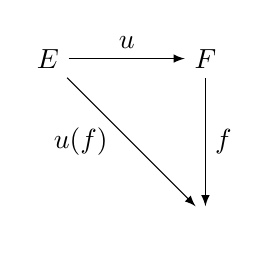
\begin{tikzpicture}
				\node (E) at (0, 0) {$E$};
				\node (F) at (2, 0) {$F$};
				\node (K) at (2, -2) {\K};
				\draw[-latex] (E) --node[above] {$u$} (F);
				\draw[-latex] (F) --node[right] {$ f $} (K);
				\draw[-latex] (E) --node[left] {$ \Star{u}(f) $\phantom{a}} (K);
			\end{tikzpicture}
		\end{center}
	% \end{figure}
	\begin{Remark}
		上一定理说明
		\[
			\varphi:\CB(E, F)\to \CB(\Star{F}, \Star{E})\qquad u\mapsto\Star{u}
		\]
		是线性等距映射, 但 $ F $ 不完备时 $ \varphi $ 不是满射.
	\end{Remark}

	\begin{Proposition}
		设 $ E, F, G $ 都是赋范线性空间, $ u\in\CB(E, F), v\in\CB(F, G) $, 则 $ (vu)^{*}=\Star{u}\Star{v} $.
	\end{Proposition}
	\begin{Proof}
		任取 $ x\in E, f\in\Star{G} $, 都有
		\[
			\lrangle{\Star{(vu)}f, x}=\lrangle{f, vu(x)}=\lrangle{\Star{v}(f), u(x)}=\lrangle{\Star{u}\Star{v}(f), x},
		\]
		从而 $ (vu)^{*}=\Star{u}\Star{v} $.\qed
	\end{Proof}

	\begin{Example}
		设 $ E $ 是赋范空间, $ F $ 是 $ E $ 的线性子空间, 记
		\[
			\varphi: F\to E\qquad x\mapsto x,
		\]
		则其共轭
		\[
			\Star{\varphi}: \Star{E}\to\Star{F}\qquad f\mapsto f|_{F}.
		\]
		特别地, 若 $ E=F $, 则 $ \varphi=\id_{E} $, 从而有 $ \Star{\id_{E}}=\id_{\Star{E}} $.
	\end{Example}	
	\begin{Theorem}
		设 $ E, F $ 是赋范空间, $ u\in\CB(E, F) $
		\begin{enumerate}[(1)]
			\item 若 $ u $ 是同构,则 $ \Star{u} $ 也是同构;
			\item 若 $ E $ 完备, 且 $ \Star{u} $ 是同构, 则 $ u $ 是同构.
		\end{enumerate}
	\end{Theorem}
	\begin{Proof}
		(1) 由 $ u $ 是同构可知 $ \exists u^{-1}\in\CB(F, E) $ 使得 $ uu^{-1}=\id_{F}, u^{-1}u=\id_{E} $, 同时对两侧取共轭, 则 $ (u^{-1})^{*}\Star{u}=\id_{\Star{F}},\Star{u}(u^{-1})^{*}=\id_{\Star{E}}  $. 从而有
		\[
			(u^{-1})^{*}=(\Star{u})^{-1},
		\]
		即 $ \Star{u} $ 的逆存在, 从而 $ \Star{u} $ 是同构.

		(2) 设 $ \Star{u} $ 是同构, 则由 (1) 可知 $ u^{**}: E^{**}\to F^{**} $ 也是同构, 则
		\[
			\forall x^{**}\in E^{**}\,\left(\frac{\norm{x^{**}}}{\norm{(u^{**})^{-1}}}\leqslant\norm{u^{**}(x^{**})}\leqslant\norm{u^{**}}\norm{x^{**}}\right).
		\]
		则 $ \forall x\in E, \forall f\in\Star{F} $, 有
		\[
			\lrangle{u^{**}(\hat{x}), f}=\lrangle{\hat{x}, \Star{u}(f)}=\lrangle{\Star{u}(f), x}=\lrangle{f, u(x)}=\langle\widehat{u(x)}, f\rangle.
		\]
		即 $ u^{**}(\hat{x})=\widehat{u(x)} $, 也即 $ u^{**}|_{E}=u $, 故有
		\[
			\forall x\in E\,\left( \frac{\norm{x}}{\norm{(u^{**})^{-1}}}\leqslant\norm{u(x)}\leqslant\norm{u}\norm{x} \right),
		\]
		则 $ u(x)=0\Longrightarrow x=0 $, 即 $ u $ 是单射, 可知 $ u^{-1} $ 在 $ u(E) $ 上有定义, 则 $ \forall y\in u(E) $ 有
		\[
			\norm{u^{-1}(y)}\leqslant\norm{(u^{**})^{-1}}\norm{y}\Rightarrow \norm{u^{-1}}\leqslant\norm{(u^{**})^{-1}}.
		\]
		由 $ E $ 完备知 $ u(E) $, 则 $ u(E) $ 在 $ F $ 中闭.

		还需说明 $ u(E)=F $. 若 $ u(E)\ne F $, 取 $ y\in F\sm u(E) $, 由 Hahn-Banach 定理, 可知 $ \exists f\in\Star{F} $ 使得 $ f|_{u(E)}=0, f(y)=1 $, 则
		\[
			\forall x\in E\,(f(u(x))=0)\Rightarrow \Star{u}(f)=0,
		\]
		因此 $ \Star{u} $ 是同构, 故只能 $ f=0 $, 矛盾, 从而 $ u(E)=F $.\qed
	\end{Proof}

	\begin{Definition}[零化子空间, 预零化子空间]\index{L!零化子空间}\index{Y!预零化子空间}\label{def:零化子空间}
		设 $ E $ 是赋范空间, $ F $ 是 $ E $ 的线性子空间, $ G $ 是 $ \Star{E} $ 的线性子空间, 称
		\[
			F^{\bot}:=\{ \Star{x}\in\Star{E}:\lrangle{\Star{x}, x}=0, \forall x\in F \}
		\]	
		为 $ F $ 的\textbf{零化子空间}, 再称
		\[
			G_{\bot}:=\{ x\in E:\lrangle{\Star{x}, x}=0, \forall \Star{x}\in G \}
		\]
		为 $ G $ 的\textbf{预零化子空间}.
	\end{Definition}

	\begin{Remark}
		因为 $ F, G $ 都是线性子空间, 则 $ F^{\bot} $ 和 $ G_{\bot} $ 分别是 $ F $ 和 $ G $ 的极, 即
		\[
			F^{\bot}=F\degree,\qquad G_{\bot}=G\degree.
		\]
		且 $ F^{\bot} $ 是 $ \Star{E} $ 中的 $ \Star{w} $--闭的线性子空间, 而 $ G_{\bot} $ 是 $ E $ 中 $ w $--闭的 (等价于范数闭的) 线性子空间, 那么双极定理~\ref{thm:双极定理}~在此对应着下面的结论:
		\[
			(F^{\bot})_{\bot}=\baro{F}^{w}=\baro{F}^{\norm{\cdot}}, \qquad (G_{\bot})^{\bot}=\baro{G}^{\Star{w}}.
		\]
	\end{Remark}

	\begin{Theorem}
		设 $ E, F $ 是赋范空间, 且 $ u\in\CB(E, F) $, 则
		\begin{enumerate}[(1)]
			\item $ \ker \Star{u}=(u(E))^{\bot} $;
			\item $ \ker u=(\Star{u}(\Star{F}))_{\bot} $;
			\item $ (\ker \Star{u})_{\bot}=\baro{u(E)}^{w}=\baro{u(E)}^{\norm{\cdot}} $;
			\item $ (\ker u)^{\bot}=\baro{\Star{u}(\Star{F})}^{\Star{w}} $.
		\end{enumerate}
	\end{Theorem}
	\begin{Proof}
		(1) 由
		\[
			\begin{aligned}
				f\in\ker\Star{u} & \Longleftrightarrow \Star{u}(f)=0 \Longleftrightarrow \forall x\in E\,(\Star{u}(f)(x)=0)\\
				& \Longleftrightarrow \forall x\in E\,(f(u(x))=0) \Longleftrightarrow \forall x\in E(\lrangle{f, u(x)}=0)\Longleftrightarrow f\in(u(E))^{\bot}.
			\end{aligned}
		\]
		可知.

		(2) 由
		\[
			\begin{aligned}
				x\in\ker u\Longleftrightarrow u(x)=0 &  \Longleftrightarrow \forall f\in\Star{F}\,(\lrangle{f, u(x)}=0)\\
				& \Longleftrightarrow \forall f\in\Star{F}\,(\lrangle{\Star{u}(f), x}=0)\Longleftrightarrow x\in(\Star{u}(F))_{\bot}
			\end{aligned}
		\]
		可知.

		(3) 因为
		\[
			(\ker\Star{u})_{\bot}=\left( (u(E))^{\bot} \right)_{\bot}=\baro{u(E)}^{w}=\baro{u(E)}^{\norm{\cdot}},
		\]
		其中最后一个等号由 Mazur 定理可证.

		(4) 由
		\[
			(\ker u)^{\bot}=\left( (\Star{u}(\Star{F}))_{\bot} \right)^{\bot}=\baro{\Star{u}(\Star{F})}^{\Star{w}}.
		\]
		可知.\qed
	\end{Proof}

	\begin{Corollary}
		设 $ E, F $ 是赋范空间, $u\in\CB(E, F)$, 则
		\begin{enumerate}[(1)]
			\item $ \Star{u} $ 是单射当且仅当 $ u(E) $ 在 $ F $ 中稠密;
			\item $ u $ 是单射当且仅当 $ \Star{u}(\Star{F}) $ 在 $ \Star{E} $ 中 $ \Star{w} $--稠密.
		\end{enumerate}	
	\end{Corollary}

\section{自反性}
	\begin{Definition}[自反空间]\index{Z!自反空间}\label{def:自反空间}
		设 $ E $ 是赋范空间, 若在自然嵌入的意义下, 有 $ E=E^{**} $, 则称 $ E $ 是一个\textbf{自反空间}.
	\end{Definition}
	\begin{Remark}
		若 $ E $ 是自反空间, 则由 $ E^{**} $ 完备可知 $ E $ 完备, 即 $ E $ 是 Banach 空间.
	\end{Remark}
	
	下面我们给出几个自反空间的例子. 前两个例子是平凡的, 即有限维赋范空间和Hilbert空间. 后两个例子与对赋范空间的讨论相同, 我们考虑一类特殊的空间, 即$ \ell_p $空间与$ L_p $空间.
	
	\begin{Proposition}
		有限维赋范空间都是自反的.
	\end{Proposition}
	\begin{Proof}
		设 $ \dim E<\infty $, 并取 $ \seq{e} $ 是一组基, 并且 $ \norm{e_{j}}=1 $, 则存在 $ \seq{f}\in\Star{E} $ 使得 $ f_{j}(e_{k})=\delta_{j, k} $, 且 $ \norm{f_{j}}=1 $, 则 $ \forall f\in\Star{E} $, 有
		\[
			f=\sum_{k=1}^{n}f(e_{k})f_{k},
		\]
		对 $ \seq{f} $, 取 $ \seq{\tilde{e}}\in E^{**} $ 使得 $ \tilde{e}_{j}(f_{k})=\delta_{j, k} $, 且 $ \norm{\tilde{e}_{j}}=1 $, 则注意到 $ \forall f\in\Star{E} $ 都有
		\[
			(\tilde{e}_{k}-\hat{e}_{k})(f)=\sum_{j=1}^{n}(\tilde{e}_{k}-\hat{e}_{k})f_{j}=\tilde{e}_{k}(f_{k})-f_{k}(e_{k})=0,
		\] 
		故 $ \tilde{e}_{k}=\hat{e}_{k} $, 则 $ \forall z\in E^{**} $ 有
		\[
			z=\sum_{k=1}^{n}z_{k}\tilde{e}_{k}=\sum_{k=1}^{n}z_{k}\hat{e}_{k}=\widehat{\sum_{k=1}^{n}z_{k}e_{k}}
		\]
		\qed
	\end{Proof}

	\begin{Proposition}
		Hilbert 空间是自反的.
	\end{Proposition}
	\begin{Proof}
		设 $ H $ 是Hilbert空间, 则由 Riesz 表示定理, 对 $ \forall \varphi\in\Star{H} $, 存在唯一的 $ y\in H $ 使得 $ \varphi(x)=\lrangle{x, y} $ 且 $ \norm{\varphi}=\norm{y} $, 不妨记其为 $ \varphi_{y} $, 则 $ \forall \varphi\in\Star{H}, \varphi=\varphi_{y} $. 于是任取 $ \varphi, \varphi'\in\Star{H} $, 有
		\[
			\lrangle{\varphi, \varphi'}:=\lrangle{\varphi_{y}, \varphi_{y'}}=\lrangle{y', y}.
		\]
		(注意到 $ \varphi_{y} $ 本身对 $ y $ 是共轭线性的, 故 $ y $ 应位于第二变元) 由此 $ \Star{H} $ 是一个 Hilbert 空间.

		而对 $ \forall f\in H^{**} $, 由 Riesz 表示定理, $ \exists\varphi_{f}\in\Star{H} $ 使得 $ \forall \varphi\in\Star{H}\,(f(\varphi)=\lrangle{\varphi, \varphi_{f}}_{\Star{H}}) $. 又存在 $ x, y\in H $ 使得 $ \varphi=\varphi_{x}, \varphi_{f}=\varphi_{y} $ 于是
		\[
			f(\varphi_{x})=\lrangle{\varphi_{x}, \varphi_{y}}=\lrangle{y, x}=\lrangle{\hat{y}, \varphi_{x}}=\hat{y}(\varphi_{x}),
		\]
		从而 $ f=\hat{y} $, 故 $ H $ 是自反的.\qed
	\end{Proof}
	
	需要注意到``括号''的性质在Banach空间上与在Hilbert空间上性质的不同. 在Hilbert空间上的内积是共轭线性的, 而在Banach空间上约定的``括号''只具有线性性.
	
	\begin{Proposition}
		设$ 1<p<\infty $, $ (p,q) $是一对共轭指数, 则$ \Star{\ell_p}\simeq\ell_q $. 另外, 有$ \Star{c_0}\simeq\ell_1 $.
	\end{Proposition}
	\begin{Proof}
		对任意的$ x\in\ell_p $, 其中$ x=(x_n)_{n\geqslant 1}=\sum\limits_{n\geqslant 1}x_ne_n $, 则
		\[
		\norm{\sum_{k=1}^nx_ke_k-x}_p=\Bnorm{\sum_{k\geqslant n+1}x_ke_k}_p=\Big(\sum_{k\geqslant n+1}\abs{x_n}^p\Big)^{1/p}\to 0,\qquad(n\to\infty)
		\]
		即$ x=\sum\limits_{n\geqslant 1}x_ne_n=\lim\limits_{n\to\infty}\sum\limits_{k=1}^nx_ke_k $. 同理, 对任意的$ x\in c_0 $, 由于
		\[
		\norm{\sum_{k=1}^nx_ke_k-x}_\infty=\sup_{k\geqslant n+1}\abs{x_k}\to 0,\qquad(n\to\infty)
		\]
		即$ x=\sum\limits_{n\geqslant 1}x_ne_n=\lim\limits_{n\to\infty}\sum\limits_{k=1}^nx_ke_k $.
		
		先证$ \ell_p $的情形, $ \forall x=(x_k)_{k\geqslant 1}\in\ell_p,\ \forall f\in\Star{\ell_p} $, 则有
		\[
		f(x)=f\Big( \sum_{n\geqslant 1}x_ne_n \Big)=\sum_{n\geqslant 1}x_nf(e_n),
		\]
		即$ f $完全由$ (f(e_n))_{n\geqslant 1} $确定, 定义
		\[
		\varphi : \Star{\ell_p}\to\ell_\infty,\qquad f\mapsto(f(e_n))_{n\geqslant 1}
		\]
		这里只将$ \ell_\infty $看作线性空间而不在其上赋范. 需要说明$ (f(e_n))_{n\geqslant 1}\in\ell_q $. 取
		\[
		x_k=\begin{cases}
		\baro{f(e_k)}\cdot\abs{f(e_k)}^{q-2} & ,1\leqslant k\leqslant n\\
		0 & , k>n\\
		\end{cases}
		\]
		则
		\[
		\begin{aligned}
		\abs{f\Big(\sum_{k\geqslant 1}x_ke_k\Big)}&=\abs{\sum_{k=1}^nx_kf(e_k)}=\sum_{k=1}^n\abs{f(e_k)}^q\\
		&\leqslant\norm{f}\cdot\Bnorm{\sum_{k\geqslant 1}x_ke_k}_p=\norm{f}\left(\sum_{k=1}^n(\abs{f(e_k)}^{q-1})^p\right)^{1/p}=\norm{f}\left(\sum_{k=1}^n\abs{f(e_k)}^q\right)^{1/p},
		\end{aligned}
		\]
		即$ \sum\limits_{k=1}^n\abs{f(e_k)}^q\leqslant\norm{f}\left(\sum\limits_{k=1}^n\abs{f(e_n)}^q\right)^{1/p} $. 注意到$ \sum\limits_{k=1}^n\abs{f(e_k)}^q\ne 0 $, 于是
		\[
		\left(\sum_{k=1}^n\abs{f(e_k)}^q\right)^{1/q}\leqslant\norm{f},
		\]
		并且注意到$ \left(\left(\sum\limits_{k=1}^n\abs{f(e_n)}^q\right)^{1/q}\right)_{n\geqslant 1} $单调递增有上界, 故其极限存在, 于是
		\[
		\norm{\varphi(f)}_q\leqslant\norm{f}<\infty,
		\]
		即$ \varphi : \Star{\ell_p}\to\ell_q $.
		
		往证$ \varphi $是等距同构, 由
		\[
		\varphi(f)=0\Longrightarrow\forall k\geqslant 1\,(f(e_k)=0)\Longrightarrow\forall x\in\ell_p\,(f(x)=0)\Longrightarrow f=0
		\]
		可知$ \varphi $是单射. 再对$ \forall y=(y_n)_{n\geqslant 1}\in\ell_q $, 定义$ f_y(x)=\sum\limits_{n\geqslant 1}x_ny_n $, 则由
		\[
		\norm{f_y(x)}\leqslant\norm{y}_q\norm{x}_p
		\]
		可知$ \norm{f_y}\leqslant\norm{y}_q<\infty $, 即$ f_y\in\Star{\ell_p} $. 注意到$ \varphi(f_y)=y $, 于是$ \varphi $是满的. 再由
		\[
		\norm{\varphi^{-1}(y)}=\norm{f_y}\leqslant\norm{y}_q
		\]
		知$ \norm{\varphi^{-1}}\leqslant 1 $. 取$ y=e_k $后$ \norm{\varphi^{-1}}=1 $, 于是$ \varphi $是等距同构, 故$ \Star{\ell_p}\simeq\ell_q $.
		
		再证$ c_0 $的情形. 对任意$ x=(x_n)_{n\geqslant 1}\in c_0 $和任意$ f\in\Star{c_0} $, 有
		\[
		f(x)=f\Big( \sum_{n\geqslant 1}x_ne_n \Big)=\sum_{n\geqslant 1}x_nf(e_n),
		\]
		取
		\[
		x_k=\begin{cases}
		\baro{f(e_k)}/\abs{f(e_k)} & ,1\leqslant k\leqslant n\,\text{且}\,f(e_k)\ne 0\\
		0 & ,k>n\,\text{或}\,f(e_k)=0
		\end{cases}
		\]
		则
		\[
		\abs{f\left(\sum_{n\geqslant 1}x_ne_n\right)}=\sum_{k=1}^n\abs{f(e_k)}\leqslant\norm{f}\norm{\sum_{k=1}^nx_ke_k}=\norm{f},
		\]
		注意到$ \left(\sum\limits_{k=1}^n\abs{f(e_k)}\right)_{n\geqslant 1} $单调递增有上界, 定义
		\[
		\varphi : \Star{c_0}\to\ell_1,\qquad f\mapsto(f(e_n))_{n\geqslant 1}
		\]
		与$ \ell_p $情形类似可证$ \varphi $是等距同构, 故$ \Star{c_0}\simeq\ell_1 $.\qed
	\end{Proof}
	
	\begin{Corollary}
		$ c_0 $不是自反的, $ \ell_p $当$ 1<p<\infty $时是自反的.
	\end{Corollary}
	
	\begin{Theorem}
		Banach空间是自反的当且仅当它的对偶也是自反的.
	\end{Theorem}
	\begin{Proof}
		\textsl{必要性.} 设$ E $是自反的Banach空间, 则$ E=E^{**} $, 从而
		\[
		(\Star{E})^{**}=E^{***}=(E^{**})^*,
		\]
		即$ \Star{E} $是自反的.
	
		\textsl{充分性.} 设$ \Star{E} $是自反的, 则有
		\[
		\Star{E}=(\Star E)^{**}=(E^{**})^*,
		\]
		假设$ E\subset E^{**} $且$ E\ne E^{**} $, 则由Hahn-Banach定理可知存在$ f\in(E^{**})^* $且$ f\ne 0 $使得$ f|_E=0 $. 又由$ (E^{**})^*=\Star{E} $可知$ f\in\Star{E} $, 且由$ f|_E=0 $可知$ f=0 $, 这与$ f\ne 0 $矛盾. 于是$ E=E^{**} $, 即$ E $是自反的.\qed
	\end{Proof}
	
	下面开始讨论$ L_p $空间的对偶, 设$ (X,\CA,\mu) $是一个$ \sigma $-有限的测度空间, 并以$ L_p $记$ L_p(X,\CA,\mu) $, $ (p,q) $是一对共轭指数.
	
	\begin{Theorem}
		设$ 1\leqslant p<\infty,\ \forall g\in L_q $, 定义
		\[
		J(g) : L_p\to\K,\qquad f\mapsto\int_Xfg\diff\mu,
		\]
		则$ J $是$ L_q $到$ \Star{L_p} $的等距同构, 即$ \Star{L_p}\simeq L_q $.
	\end{Theorem}
	\begin{Proof}
		只证$ \K=\C $的情形, 先说明$ J $是等距的. 由H\"older不等式
		\[
		\abs{J(g)(f)}=\abs{\int_Xfg\diff\mu}\leqslant\norm{f}_p\norm{g}_q,
		\]
		从而$ \norm{J(g)}\leqslant\norm{g}_q $, 可知$ \norm{J}\leqslant 1 $.
	
		当$ p>1 $时取$ f=\frac{\bar{g}}{\abs{g}}\cdot\frac{\abs{g}^{q-1}}{\norm g_q^{q-1}} $, 则因
		\[
		\int_X\abs{f}^p\diff\mu=\int_X\frac{(\norm{g}^{q-1})^p}{(\norm{g}_q^{q-1})^p}\diff\mu=\frac{1}{\norm{g}_q^q}\int_X\abs{g}^q\diff\mu=\frac{\norm{g}_q^q}{\norm{g}_q^q}=1,
		\]
		知$ \norm{f}_p^p=1 $, 从而$ \norm{f}_p=1 $, 且
		\[
		\abs{J(g)(f)}=\abs{\int_Xfg\diff\mu}=\int_X\frac{\abs{g}^q}{\norm{g}_q^{q-1}}\diff\mu=\norm{g}_q,
		\]
		即$ \norm{J(g)}\geqslant\norm{g}_q $可知$ \norm{J}\geqslant 1 $, 于是$ \norm{J}=1 $, 即$ J $是等距的.
	
		当$ p=1 $时, 取$ A_\varepsilon=\{ x : \abs{g(x)}\geqslant\norm		g_\infty-\varepsilon \} $. 由本性上确界的定义可知$ \mu(A_\varepsilon)\ne 0 $. 因为$ \mu $是$ \sigma $-有限的, 不妨设$ \mu(A_\varepsilon)<\infty $. 令$ f_\varepsilon=\frac{1}{\mu(A_\varepsilon)}\cdot\frac{\bar{g}}{\abs{g}}1_{A_\varepsilon} $, 则$ \norm{f_\varepsilon}_1=1 $, 且
		\[
		\abs{J(g)(f_\varepsilon)}=\frac{1}{\mu(A_\varepsilon)}\int_{A_\varepsilon}\frac{\bar{g}}{\abs{g}}g\diff\mu\geqslant\frac{1}{\mu(A_\varepsilon)}(\norm{g}_\infty-\varepsilon)\mu(A_\varepsilon)=\norm{g}_\infty-\varepsilon,
		\]
		由$ \varepsilon $的任意性可知$ \norm{J(g)}\geqslant\norm{g}_\infty $, 即$ \norm{J}\geqslant 1 $, 于是$ J $是等距的.
	
		由
		\[
		\abs{J(g)}=0\Longrightarrow\forall f\in L_p\,\left(\int_Xfg\diff\mu=0\right)\Longrightarrow g=0
		\]
		可知$ J $是单射, 还需说明$ J $是满射. $ \forall \varphi\in\Star{L_p},\ \exists g\in L_q $使得$ J(g)=\varphi $, 定义集函数$ \nu $使得对任意$ \mu $-有限的可测集$ A\subset X $, 都有
		\[
		\nu(A)=\varphi(1_A),
		\]
		则由可测函数的简单逼近性质和$ \nu $的可列加性可知$ \nu $是一个复测度, 对使得$ \mu(A)=0 $的可测集$ A $, 有
		\[
		\abs{\nu(A)}=\abs{\varphi(1_A)}\leqslant\norm{\varphi}\int_X1_A\diff\mu=\norm{\varphi}\mu(A)=0
		\]
		于是$ \nu(A)=0 $. 这说明$ \nu $依$ \mu $绝对连续. 由Radon-Nikodym定理, 存在可测函数$ g $使得$ \diff\nu=g\diff\mu $. 下证$ g\in L_q $.
	
		形式上, 有$ \varphi(f)=\int_Xfg\diff\mu $, 当$ 1<p<\infty $时, 令$ E_n=\{ x : \abs{g(x)}\leqslant n \} $, 并令$ f=1_{E_n}\abs{g}^{q-2}\bar{g} $. 则
		\[
		\int_{E_n}\abs{g}^q\diff\mu=\int_Xfg\diff\mu=\varphi(f)\leqslant\norm{\varphi}\cdot\norm{f}_p=\norm{\varphi}\left(\int_{E_n}\abs{g}^q\diff\mu\right)^{1/p}
		\]
		即
		\[
		\left(\int_{E_n}\abs{g}^q\diff\mu\right)^{1-1/p}=\left( \int_{E_n}\abs{g}^q\diff\mu \right)^{1/q}\leqslant\norm{\varphi},
		\]
		令$ n\to\infty $, 注意到$ ((\int_{E_n}\abs{g}^q\diff\mu)^{1/q})_{n\geqslant 1} $单调递增有上界, 故极限存在. 则$ \norm{g}_q\leqslant\norm{\varphi}<\infty $, 故$ g\in L_q $.
	
		当$ p=1 $时, $ q=\infty $, 作$ A_\varepsilon=\{ x : \abs{g(x)}\geqslant\norm{\varphi}+\varepsilon \} $, 往证$ \mu(A_\varepsilon)=0 $. 取$ f=1_{E_n}\cdot1_{A_\varepsilon}\cdot\frac{\bar{g}}{\abs{g}} $, 则$ \norm{f_n}_1=\int_{E_n\cap A_\varepsilon}1\diff\mu=\mu(E_n\cap A_\varepsilon) $, 则
		\[
		\varphi(f_n)=\int_{A_\varepsilon\cap E_n}\abs{g}\diff\mu\geqslant(\norm{\varphi}+\varepsilon)\mu(E_n\cap A_\varepsilon),
		\]
		又
		\[
		\abs{\varphi(f_n)}\leqslant\norm{\varphi}\norm{f_n}_1=\norm{\varphi}\cdot\mu(E_n\cap A_\varepsilon),
		\]
		于是
		\[
		(\norm{\varphi}+\varepsilon)\mu(E_n\cap A_\varepsilon)\leqslant\norm{\varphi}\cdot\mu(E_n\cap A_\varepsilon)
		\]
		只能$ \mu(E_n\cap A_\varepsilon)=0 $, 令$ n\to\infty $就有$ \mu(A_\varepsilon)=0 $. 从而$ \norm{g}_\infty\leqslant\norm{\varphi}<\infty $, 即$ g\in L_\infty $.\qed
	\end{Proof}
	
	\begin{Corollary}
		$ L_p(X,\mu) $在$ 1<p<\infty $时是自反的.
	\end{Corollary}
	
\section{弱*紧性}
	
	\begin{Theorem}[Banach-Alaoglu]
	设$ E $是赋范空间, 则$ \bar{B}_{\Star{E}} $是$ w^* $--紧的.
	\end{Theorem}
	\begin{Proof}
	\textsl{这是一个不正式的证明.}
	
	对$ f\in\bar{B}_{\Star{E}} $, 有$ f : E\to\C $使得$ \abs{f(x)}\leqslant\norm{x} $. 定义$ D_x=\{ z\in\C : \abs{z}\leqslant\norm{x} \} $, 下面建立$ f $与$ \prod\limits_{x\in E}D_x $的映射. 定义
	\[
	\varPhi : \bar{B}_{\Star{E}}\to\prod_{x\in E}D_x,\qquad f\mapsto(f(x))_{x\in E},
	\]
	这是一个单射, 往证$ \varPhi $与$ \varPhi^{-1} $都连续.
	
	(方法1, 使用开集的方式) 取$ D_{x_0} $中的开圆盘$ B(y_0,r) $, 则$ \prod\limits_{x\ne x_0}D_x\times B(y_0,r) $是一个基础开集, 则其在$ \varPhi $下的原像
	\[
	\{ f : \abs{f(x_0)-y_0}<r \}
	\]
	是$ w^* $--拓扑下的开集. 更一般地, 考虑有限个开圆盘$ B(y_i,r_i)\subset D_{x_i} $, 其中$ i=1,2,\dots,n $, 则$ \prod\limits_{x\ne x_j}D_x\times\prod\limits_{i=1}^nB(y_i,r_i) $的原像
	\[
	\{ f : \abs{f(x_i)-y_i}<r_i,\ \forall i = 1,2,\dots,n \}
	\]
	是$ w^* $--拓扑下的开集, 故$ \varPhi $是连续的.
	
	注意到$ \varPhi(\bar{B}_{x\in E}) $是由$ \prod\limits_{\Star{E}}D_x $的乘积拓扑限制得到, 取$ \bar{B}_{\Star{E}} $中$ w^* $--拓扑开集
	\[
	V(f_0,\seq{x},\varepsilon):=\{ f : \abs{f(x_i)-f_0(x_i)}<\varepsilon_i,\ \forall i=1,2,\dots,n \}
	\]
	则
	\[
	\varPhi(V(f_0,\seq{x},\varepsilon))=\varPhi(\bar{B}_{\Star{E}})\cap\left(\prod_{x\ne x_j}D_x\times\prod_{i=1}^nB(f_0(x_i),\varepsilon_i)\right)
	\]
	是开集, 故$ \varPhi^{-1} $是连续的.
	
	(方法2, 使用网的极限) 取$ (f_i)_{i\uparrow\alpha} $是$ \bar{B}_{\Star{E}} $中的网, 且$ f_i\sweakto f $, 则
	\[
	\forall x\in E\,(f_i(x)\to f(x))\Longrightarrow (f_i(x))_{x\in E}\to(f(x))_{x\in E}
	\]
	故$ \varPhi $连续. 反之, 再在$ \bar{B}_{\Star{E}} $中取$ (f_i(x))_{x\in E}\to (f(x))_{x\in E} $, 则
	\[
	\forall x\in E\,(f_i(x)\to f(x))\Longrightarrow f_i\sweakto f.
	\]
	故$ \varPhi^{-1} $连续.
	
	往证$ \varPhi(\bar{B}_{\Star{E}}) $是$ \prod\limits_{x\in E}D_x $中的闭集(\textsl{这一结果并非平凡的}). 因为
	\[
	\begin{aligned}
	\varPhi(\bar{B}_{\Star{E}})&=\left\{ (g_x)_{x\in E}\in\prod_{x\in E}D_x : g_{ax+by}=ag_x+bg_y,\ \forall a,b\in\C,\ \forall x,y\in E \right\}\\
	&=\bigcap_{a,b\in\C}\bigcap_{x,y\in E}\left\{ (g_x)_{x\in E}\in\prod_{x\in E}D_x : g_{ax+by}=ag_x+bg_y \right\}
	\end{aligned}
	\]
	若有$ (g_x^{(i)})_{x\in E} $在$ \prod\limits_{x\in E}D_x $中收敛到$ (g_x)_{x\in E} $, 则
	\[
	\begin{aligned}
	\forall x\in E(g_x^{(i)}\to g(x))&\Longrightarrow g_{ax'+by'}^{(i)}=ag_{x'}^{(i)}+bg_{y'}^{(i)}\\
	&\Longrightarrow g_{ax'+by'}=ag_{x'}+bg_{y'}\Longrightarrow g_x\in\varPhi(\bar{B}_{\Star{E}})
	\end{aligned}
	\]
	即$ \varPhi(\bar{B}_{\Star{E}}) $是闭的. 由Tychonoff定理可知$ \prod\limits_{x\in E}D_x $紧, 从而$ \varPhi(\bar{B}_{\Star{E}}) $也是紧的, 于是$ \bar{B}_{\Star{E}} $是$ w^* $--紧的.\qed
	\end{Proof}
	
	\begin{Corollary}
	设$ H $是Hilbert空间, 则$ \bar{B}_H $是$ w $--紧的.
	\end{Corollary}
	
	\begin{Theorem}[Goldstine]
	设$ E $是赋范空间, 则$ \bar{B}_E^{\Star{w}}=\bar{B}_{E^{**}} $.
	\end{Theorem}
	
	这一定理的证明超出本课程要求, 此处略去.
	
	\begin{Corollary}[Banach]
	设$ E $是赋范空间, 则$ E $是自反的当且仅当$ \bar{B}_E $是$ w $--紧的.
	\end{Corollary}
	\begin{Proof}
	\textsl{必要性}. 由$ E $是自反的可知$ E=E^{**} $, 从而$ \bar{B}_E=\bar{B}_{E^{**}} $. 由Banach-Alaoglu定理可知$ \bar{B}_{E^{**}} $是$ w $--紧的, 于是$ \bar{B}_E $是$ w $--紧的.
	
	\textsl{充分性}. 由$ \bar{B}_E $是$ w $--紧的可知$ \bar{B}_E\hookrightarrow\bar{B}_{E^{**}} $, 因为 $ \bar{B}_{E^{**}} $ 是$ \Star{w} $--紧的, 故$ \bar{B}_E $是$ \Star{w} $--紧的. 则$ \bar{B}_E $在$ \bar{B}_{E^{**}} $中$ \Star{w} $--闭, 即$ \bar{B}_E=\bar{B}_E^{\Star{w}} $. 由Goldstine定理可知$ \bar{B}_E^{\Star{w}}=\bar{B}_{E^{**}} $, 从而$ \bar{B}_E=\bar{B}_{E^{**}} $, 这说明$ E=E^{**} $, 即$ E $是自反的.\qed
	\end{Proof}
	
	\begin{Remark}
	在$ E $上有三种拓扑, 其中范数拓扑强于弱拓扑, 而弱拓扑强于弱*拓扑. 在三种拓扑下$ \Star{E} $的单位球的紧性对应了$ E $的不同性质. 其中$ \bar{B}_{\Star{E}} $紧等价于$ \dim \Star{E}<\infty $, 进一步等价于$ \dim E<\infty $. 而$ \bar{B}_{\Star{E}} $$ w $--紧当且仅当$ \Star{E} $是自反的, 它等价于$ E $是自反的. 而$ \bar{B}_{\Star{E}} $总是$ \Star{w} $--紧的.
	\end{Remark}
	
\section*{本章习题}
	\addcontentsline{toc}{section}{本章习题}
	
	习题后面括号中的序号表示对应书中习题的编号.
	
	\begin{enumerate}[label=\textbf{\arabic*.}, ref=\arabic*]
		\item (补充7) 设 $ E $ 是\R 上的赋范空间, $ \varOmega $ 是 $ E $ 中原点处的吸收凸邻域, $ p_{\varOmega} $ 是 $ \varOmega $ 上的 Minkowski 泛函, 验证 $ p_{\varOmega} $ 是 $ E $ 上的次线性泛函.
		\item (8.1) 设 $ 1\leqslant p\leqslant\infty $, 考虑 $ \R^{2} $ 上的 $ p $ 范数:
			\[
				\norm{(x_{1}, x_{2})}_{p}=
				\begin{cases}
					\big( \abs{x_{1}}^{p}+\abs{x_{2}}^{p} \big)^{1/p} & ,p<\infty\\
					\max\{\abs{x_{1}}, \abs{x_{2}}\} & ,p = \infty
				\end{cases}
			\]
			设 $ F=\R\times\{ 0 \} $, 即由 $ e_{1}=(1, 0) $ 生成的线性子空间, 并设 $ f:F\to\R $ 是线性泛函, 满足 $ f(e_{1})=1 $.
			\begin{enumerate}[(1)]
				\item 当 $ \R^{2} $ 上赋予 $ \norm{\cdot}_{1} $ 范数时, 确定 $ f $ 从 $ F $ 到 $ \R^{2} $ 的所有保范延拓;
				\item 当 $ \R^{2} $ 上赋予 $ \norm{\cdot}_{p} $ 范数时, 考虑同样的问题.
			\end{enumerate}
		\item (补充8) 判断 $ (\R^{2}, \norm{\cdot}_{p}), 1\leqslant p\leqslant\infty $ 的严格凸性.
		\item (8.3) 设$ E $是数域$ \K $上的赋范空间, $ A\subset E $, 并设$ f : A\to\K $以及常数$ \lambda\geqslant 0 $. 证明: 存在$ \hat{f}\in\Star{E} $使得
			\[
			(\hat{f}\rvert_A=f)\land (\tnorm{\hat{f}}\leqslant\lambda)
			\]
			的充分必要条件是
			\[
			\abs{\sum_{k=1}^n\alpha_kf(a_k)}\leqslant\lambda\norm{\sum_{k=1}^n\alpha_ka_k}
			\]
			对任意$ n\in\N $, $ (\seq{a})\in A^n $, $ (\seq{\alpha})\in\K^n $成立.
		\item (8.4) 设$ E $是Hausdorff拓扑向量空间, $ A $是$ E $中包含原点的开凸集且$ x_0\in E\sm A $.
			\begin{enumerate}[(1)]
			\item 证明: 存在$ f\in\Star{E} $使得$ \Re f(x_0)=1 $且在$ A $上成立$ \Re f<1 $.
			\item 假设$ A $还是平衡的. 证明: 可以选择$ f\in\Star{E} $满足$ f(x_0)=1 $且在$ A $上成立$ \abs{f}<1 $.
			\end{enumerate}
		\item (8.9) 设$ E $是数域$ \K $上的拓扑向量空间, 称$ E $的线性子空间$ H $是超平面, 若存在$ x_0\in E\sm H $使得$ E=H+\K x_0 $.
			\begin{enumerate}[(1)]
			\item 证明: 若$ H $是超平面, 则对任意$ x\in E\sm H $, 都有$ E=H+\K x $成立.
			\item 证明: 一个超平面或者是$ E $中的稠密集, 或者是$ E $中的闭集.
			\item 证明: $ H $是超平面当且仅当存在$ E $上的一个非零线性泛函使得$ H=\ker f $. 因而$ H $是闭的等价于$ f $是连续的.
			\end{enumerate}
		\item (8.13) 考虑空间$ \ell_1 $中的如下子集:
			\[
			\begin{aligned}
			A_0&=\{ x=(x_n)_{n\geqslant 1}\in\ell_1 : x_{2n}=0,\ \forall n\geqslant 1 \}\\
			B&=\{ x=(x_n)_{n\geqslant 1}\in\ell_1 : x_{2n}=2^{-n}x_{2n-1},\ \forall n\geqslant 1 \}.
			\end{aligned}
			\]
			\begin{enumerate}[(1)]
			\item 证明: $ A_0 $与$ B $都是$ \ell_1 $的闭线性子空间, 且$ A_0+B $在$\ell_1 $中稠密;
			\item 设$ c\in\ell_1 $满足$ c_{2n-1}=0 $及$ c_{2n}=2^{-n} $, 并设$ A=A_0-c $. 证明: $ c\notin A_0+B $且$ A\cap B=\varnothing $, 并证明: 不存在非零的$ f\in\Star{\ell_1} $和$ \alpha\in\R $使得$ A\subset\{ f\leqslant\alpha \} $且$ B\subset\{ f\geqslant\alpha \} $.
			\end{enumerate}
		\item (8.15) 本习题的目的是刻画连续线性泛函的 Hahn-Banach 延拓的唯一性问题. 设 $ E $ 是一个维数至少为 2 的赋范空间, 证明: $ E $ 的线性子空间 $ F $ 上的每个连续线性泛函有唯一的保范延拓的充分必要条件是 $ \Star{E} $ 是严格凸的.
		\item (8.16) 考虑空间 $ \ell_{\infty} $ 和它的线性子空间 $ F $:
			\[
				F = \left\{ x\in\ell_{\infty}:\lim_{n\to\infty} m_{n}(x)\ \text{存在} \right\}, \qquad m_{n}(x)=\frac{1}{n}\sum_{k=1}^{n} x_{k}.
			\]
			\begin{enumerate}[(1)]
				\item 定义 $ f:F\to\R $ 为 $ f(x)=\lim\limits_{n\to\infty}m_{n}(x) $. 证明 $ f\in\Star{F} $.
				\item 证明: 存在 $ \ell_{\infty} $ 上的连续线性泛函 $ m $ 满足下面的性质:
				\begin{enumerate}[(i)]
					\item $ \liminf\limits_{n\to\infty}x_{n}\leqslant m(x)\leqslant\limsup\limits_{n\to\infty}x_{n}, \qquad x\in\ell_{\infty} $.
					\item $ m\circ \tau=m $, 这里 $ \tau: \ell_{\infty}\to\ell_{\infty} $ 是左移算子, 即 $ (\tau(x))_{n}=x_{n+1} $. ($ m $ 被称为 Banach 平均或 $ \ell_{\infty} $--极限.)
				\end{enumerate}
			\end{enumerate}
		\item (8.21) 设$ e_n(t)=\exp(\imag nt) $, 其中$ t\in[0,2\pi] $.
		\begin{enumerate}[(1)]
			\item 证明: 对每个$ 1\leqslant p<\infty $, $ (e_n)_{n\geqslant 1} $在$ L_p(0,2\pi) $中弱收敛到0但不依范数收敛到0.
			\item 设$ f_n=\frac{1}{n}\sum\limits_{k=1}^{n^2}e_k $. 证明: $ (f_n)_{n\geqslant 1} $在$ L_2(0,2\pi) $中弱收敛到0但不依范数收敛到0.
		\end{enumerate}
		\item (9.1) 设 $ E $ 是赋范空间, 并设 $ \Star{E} $ 是可分的.
		\begin{enumerate}[(1)]
			\item 令 $ (f_{n})_{n\geqslant1} $ 是 $ \Star{E} $ 中的稠密子集. 选出 $ E $ 中的序列 $ (x_{n})_{n\geqslant1} $ 使得 $ f_{n}(x_{n})\geqslant \norm{f_{n}}/2 $.
			\item 任取 $ f\in\Star{E} $. 证明: 若对每个 $ x_{n} $ 有 $ f(x_{n})=0 $, 则 $ f=0 $. 
			\item 由此导出 $ \Span(x_{1}, x_{2}, \dots) $ 在 $ E $ 中稠密且 $ E $ 是可分的.
			\item 证明: 一个 Banach 空间是可分且自反的当且仅当它的对偶空间是可分且自反的.
			\item 举一个可分赋范空间但其对偶空间不可分的例子. 
		\end{enumerate}
		\item (9.2) 设$ E $是Banach空间, $ B\subset\Star{E} $
		\begin{enumerate}[(1)]
			\item 证明: $ B $是相对$ \Star{w} $--紧的当且仅当$ B $是有界的.
			\item 假设 $ B $ 是有界的且 $ E $ 是可分的. 证明: $ (B, \sigma(\Star{E}, E)) $ 可度量化.
		\end{enumerate}
		\item (9.4) 设 $ E $ 是自反空间, 证明: $ E $ 中的每个有界序列 $ (x_{n})_{n\geqslant1} $ 有弱收敛子序列.
		\item (9.6a) 令$ E $和$ F $是两个Banach空间, 且$ u\in\CB(E,F) $. 证明: $ u $是从$ E $到$ F $的满的等距映射当且仅当$ \Star{u} $是$ \Star{F} $到$ \Star{E} $的满的等距映射.
		\item (9.8) 设$ P $是Banach空间$ X $上的线性映射并满足$ P\circ P=P $, 记$ R=P(X) $且$ N=\ker P $.
		\begin{enumerate}[(1)]
			\item 证明: $ X=R\oplus N $, 再证明$ P $连续的充分必要条件是$ R $和$ N $都是闭集.
			\item 假设$ P $是连续的, 证明: $ R^\bot $和$ N^\bot $在$ \Star{X} $中互补, 且有$ \Star{X}=R^\bot\oplus N^\bot $.
		\end{enumerate}
		\item (9.16) 称 Banach 空间 $ E $ 为\textbf{一致凸}\index{Y!一致凸}的, 若对任意 $ \varepsilon>0 $, 存在 $ \delta>0 $, 使得
		\[
			\forall x, y\in\bar{B}_{E}\,\left(\norm{x-y}\geqslant\varepsilon\Rightarrow \norm{\frac{x+y}{2}}\leqslant 1-\delta\right).
		\]
		设 $ (x_{n})_{n\geqslant1} $ 是一致凸空间 $ E $ 中弱收敛到 $ x $ 的序列, 并有 $ \lim\limits_{n\to\infty}\norm{x_{n}}=\norm{x} $. 证明 $ (x_{n})_{n\geqslant1} $ 依范数收敛到 $ x $. 用例子说明条件 $ \lim\limits_{n\to\infty}\norm{x_{n}}=\norm{x} $ 是必需的.
	\end{enumerate}